\documentclass[useAMS,usenatbib]{mnras}
% \documentclass[fleqn,usenatbib,letters]{mnras}

\usepackage{epsfig,bm}
\usepackage{amsbsy,amssymb,amsmath}
\usepackage{graphicx}
\usepackage{dcolumn}

% \usepackage[T1]{fontenc}
% \usepackage{ae,aecompl}
% % \usepackage[font=small,belowskip=0pt]{caption}
% \usepackage{interval}  %for prior intervals
% \usepackage{relsize}
% \usepackage{balance}

\usepackage{float}
% \usepackage{color}
\usepackage[usenames,dvipsnames]{xcolor}
\usepackage{hyperref}
\hypersetup{
    colorlinks = true,
    citecolor = {MidnightBlue},
    linkcolor = {BrickRed},
    urlcolor = {BrickRed}
}

\usepackage{ctable}
\usepackage{caption}


\newcommand{\grad}{\ensuremath{\vec{\nabla}}}
\newcommand{\be}{\begin{equation}}
\newcommand{\ee}{\end{equation}}
\newcommand{\bea}{\begin{eqnarray}}
\newcommand{\eea}{\end{eqnarray}}
\newcommand{\bL}{\mathbf{L}}
\newcommand{\bl}{\mathbf{l}}
\newcommand{\kpe}{k_\perp}
\newcommand{\kpa}{k_\parallel}
\newcommand{\cb}{\color{blue}}
\newcommand{\bn}{\mathbf{n}}
\newcommand{\ama}[1]{\textcolor{red}{{#1}}}



\title[Magnification measurements with HI intensity mapping]
{Prospects for cosmic magnification measurements using HI intensity mapping}

\begin{document}

\maketitle

\begin{abstract}
We investigate the prospects of measuring the cosmic magnification effect by cross-correlating 21cm intensity mapping (HI IM) foreground maps with background optical galaxies. We forecast the signal-to-noise ratio for HI IM data from SKA1 MID and HIRAX, combined with LSST photometric galaxy samples. We find that, thanks to their different resolutions, SKA and HIRAX are highly complementary in such an analysis. A future detection by either of these instruments would achieve a cumulative signal-to-noise ratio of $\sim 5-10$ on disjoint multipole ranges. This would allow measurements of the magnification signal on a wide redshift range with foreground maps at up to $z \lesssim xxx$ \ama{finalize}.
\end{abstract}

\begin{keywords}
cosmology: large-scale structure of the universe
\end{keywords}

%\section{Introduction}
%The plan of the paper is as follows: In Section~\ref{sec:formalism} [...]


\section{Introduction}
Traveling through our universe, the path of light is bent by the mass and energy distribution it encounters. Images of distant light sources are distorted by the intervening matter along the line of sight (LOS), an effect well described by the General Theory of Relativity. Distortions of shapes, magnifications and even duplicate images are observed and generally classified as weak or strong gravitational lensing. A particularly weak form of lensing, cosmic magnification, can be measured even when the sizes and shapes of sources are inaccessible. Magnification occurs when intervening structure between an observer and a source acts to magnify or demagnify the object, i.e. sometimes allowing the observer to see objects otherwise too faint. However, the apparent observed area can also be increased, which leads to an apparent decrease in number counts if the total number is conserved. Only slightly altering the observed structures, this effect is notoriously difficult to measure \citep[e.g.][]{2009A&A...507..683H, 0004-637X-814-2-145, 2008PhRvD..78l3517Z, 2006MNRAS.367..169Z}. Several promising techniques exist, but until now it has only seen few detections, one such is the $8\sigma$ detection achieved in \citet{2005ApJ...633..589S} using the Sloan Digital Sky Survey and the galaxy-quasar cross-correlation. Measurements of cosmic magnification probe the galaxy halo occupation distribution, dark matter halo ellipticities and the extent of galaxy dust halos. Similar to weak lensing, it also provides constraints on galaxy-matter correlation, but without the requirement of measuring shapes, it suffers from less systematic errors and can be extended to sources at much higher redshifts \citep{2005ApJ...633..589S}. In addition to probing the matter distribution directly, magnification also plays an important role in \emph{geometrical methods} to measure dark energy parameters independently of the matter power spectrum \citep{2007MNRAS.374.1377T,2004ApJ...600...17B,2003PhRvL..91n1302J}. These methods use galaxy-lensing correlations and therefore depend on estimates of the galaxy density. This is directly affected by magnification, which can therefore introduce systematic errors unless corrected for \citep{2005ApJ...633..589S}.

A straightforward approach to measure magnification uses the angular cross-correlation between foreground and background galaxy counts, where galaxy-magnification or magnification-magnification cross-correlations would be major contributors to a non-zero signal. Following a similar line of thought, we propose to use HI intensity maps acting as lenses, magnifying a background distribution of galaxies. The intensity maps are unresolved, and therefore not magnified themselves by the matter between them and the observer, which removes magnification-magnification correlations between foreground and background. This potentially decreases the signal, but also helps interpretation by removing additional terms in the signal calculation. The extremely high redshift resolution of the foreground HI maps allows to combine measurements using different slices of the HI distribution and thus significantly improves the expected signal to noise. In the following, we derive forecasts for a potential detection of the magnification signal, using noise properties for the planned radio telescopes SKA1 and HIRAX, as well as LSST.


\section{Cosmic magnification}
\subsection{Galaxies as foregrounds}
\label{ssec:maggal}
% Using galaxies as biased tracers of matter, cosmic magnification is the effect of lensing in the observed galaxy distribution. Lensing magnification makes galaxies appear brighter, which means that objects that are dimmer than the flux cutoff of a given survey can be detected, so that their observed number density  increases. However, the apparent area is also increased, therefore the observed number density of galaxies decreases. Formalising the above description we can write the observed galaxy number overdensity as \citep{2008PhRvD..78l3517Z}
Galaxies are biased tracers of the underlying dark matter distribution, which is thought to contain most of the mass distributed along the LOS to a light source. Magnification will increase the flux from a galaxy, making it appear brighter than it actually is. Therefore galaxies normally too faint to be detected can still be seen if the magnification caused by the matter along the LOS is strong enough. However, the apparent area of a source is also increased, resulting in a decrease of the observed number density of galaxies. Following the description in \citep{2008PhRvD..78l3517Z}, one can write
\be
\delta^{\rm L}_{\rm g}=\delta_{\rm g}+(5s_{\rm g}-2)\kappa +\mathcal{O}(\kappa^2) \, ,
\ee with $\delta_{\rm g}^{\rm L}$ and $\delta_{\rm g}$ the lensed and unlensed intrinsic galaxy over-densities, respectively, and $\kappa$ the lensing convergence. For a survey with limiting magnitude $m^\star$ the number count slope $s_{\rm g}$ is given by
\be
\label{eq:sg}
s_{\rm g} = \frac{d{\rm \, log}_{10}N(< m^\star)}{dm^\star} \, .
\ee
The cross-correlation of well separated foreground (at position $\Theta_{\rm f}$ and redshift $z_{\rm f}$) and background ($\Theta_{\rm b}$ and $z_{\rm b}$) galaxy samples is independent of the intrinsic galaxy over-density correlation term $\langle \delta_{\rm g}(\theta_{\rm f},z_{\rm f}) \delta_{\rm g}(\theta_{\rm b},z_{\rm b}) \rangle$, therefore
\bea
\label{eq:magcorr}
\langle \delta^{\rm L}_{\rm g}(\theta_{\rm f},z_{\rm f}) \delta^{\rm L}_{\rm g}(\theta_{\rm b},z_{\rm b}) \rangle
&=& \langle(5s^{\rm b}_{\rm g}-2) \kappa_{\rm b}  \delta_{\rm g}(\theta_{\rm f},z_{\rm f}) \rangle \nonumber \\
&+& \langle(5s^{\rm f}_{\rm g}-2)(5s^{\rm b}_{\rm g}-2)  \kappa_{\rm f} \kappa_{\rm b} \rangle \, ,
\eea
where the superscript ${}^{\rm L}$ denotes lensed quantities. The right hand side of equation \ref{eq:magcorr} contains the magnification-galaxy ($\mu-\rm g$) correlation (first term) and the magnification-magnification ($\mu-\mu$) correlation (second term). The latter is subdominant for foregrounds at comparably low redshifts and therefore usually neglected. If both foreground and background galaxies are at high redshifts, however, it can become large \citep{2008PhRvD..78l3517Z}.

% Measurements of the $\mu g$ correlation are useful to constrain the galaxy-mass power spectrum. The method is complementary to galaxy-galaxy shear measurements, being free from many systematic errors that affect shear measurements such as point spread function and galaxy intrinsic alignment.

\subsection{Cosmic magnification with HI intensity mapping}

In this work, we focus on the magnification effect of HI intensity maps in the foreground, acting on the clustering statistics of background galaxies. Intensity maps themselves are not lensed at linear order due to surface brightness conservation \citep{PhysRevD.87.064026}. Assuming an HI foreground and a galaxy background sample as dark matter tracers, it follows thus that $s_{\rm HI} = 2/5$ and
\be
\delta T^{\rm L}_{21}=\delta T_{21}=\bar{T}_{21} \delta_{\rm HI} = \bar{T}_{21} b_{\rm HI} \delta \, ,
\ee where $\bar{T}_{21}$ is the mean brightness temperature of neutral hydrogen, $b_{\rm HI}$ is the hydrogen bias and $\delta$ the dark matter over-density. Therefore
\be
\langle \delta^{\rm L}_{\rm HI}(\theta_{\rm f},z_{\rm f}) \delta^{\rm L}_{\rm g}(\theta_b,z_b) \rangle
= \langle (5s^{\rm b}_{\rm g}-2) \kappa_b  b_{\rm HI} \delta (\theta_{\rm f},z_{\rm f}) \rangle \, .
\ee
Note the absence of the magnification-magnification term since $s_{\rm HI}=2/5$. Therefore the above relation is exact at all redshifts, given that the foreground and background samples are well separated. This can be guaranteed via the excellent redshift information provided by the intensity mapping survey.



The observable magnification signal can be expressed using the angular power spectrum \citet{2008PhRvD..78l3517Z}
\bea
\label{eq:clhimu}
&&C^{{\rm HI} - \mu}_\ell (z_{\rm f}, z_{\rm b}) = \frac{3}{2}\frac{H^2_0}{c^2}\Omega_{{\rm m},0} \times  \nonumber \\
&& \int^{\infty}_0 dz \frac{b_{\rm HI}\bar{T}_{21}(z)W(z,z_{\rm f})g(z,z_{\rm b})}{r^2(z)}(1+z) \times \nonumber \\ 
&& P((\ell+1/2)/r(z),z) \, ,
\eea
where we have applied the Limber approximation, valid for $\ell \geq 10$ \citep{1954ApJ...119..655L,2008PhRvD..78l3506L}. Here the redshift distribution of the foreground sources is given by the top hat over the foreground redshift bin $W(z,z_{\rm f})$ and $g(z,z_{\rm b})$ is the lensing kernel:
\be
g(z,z_{\rm b})=\frac{r(z)}{N_{\rm g}(z_{\rm b})}\int^{z_{\rm b}^{\rm max}}_{z_{\rm b}^{\rm min}} dz' \frac{r(z')-r(z)}{r(z')}(5s_{\rm g}(z')-2)n_{\rm g}(z') \, ,
\label{eq:gkernel}
\ee
where the number of galaxies per square degree in the background bin is
\be
N_{\rm g}(z_{\rm b}) \equiv \int_{z_{\rm b}^{\rm min}}^{z_{\rm b}^{\rm max}} n_{\rm g}(z)dz.
\label{eq:ngNg}
\ee

 The number count slope $s_{\rm g}$ is shown in \ref{fig:sg}, while figure \ref{fig:gkernel} presents it in the context of the integration for the lensing kernel $g$. The magnitude threshold can be chosen to avoid a sign change of $5s_{\rm g} -2$ in the background redshift bin, which boosts the signal by avoiding cancellations inside the integral.

\begin{figure}
\centering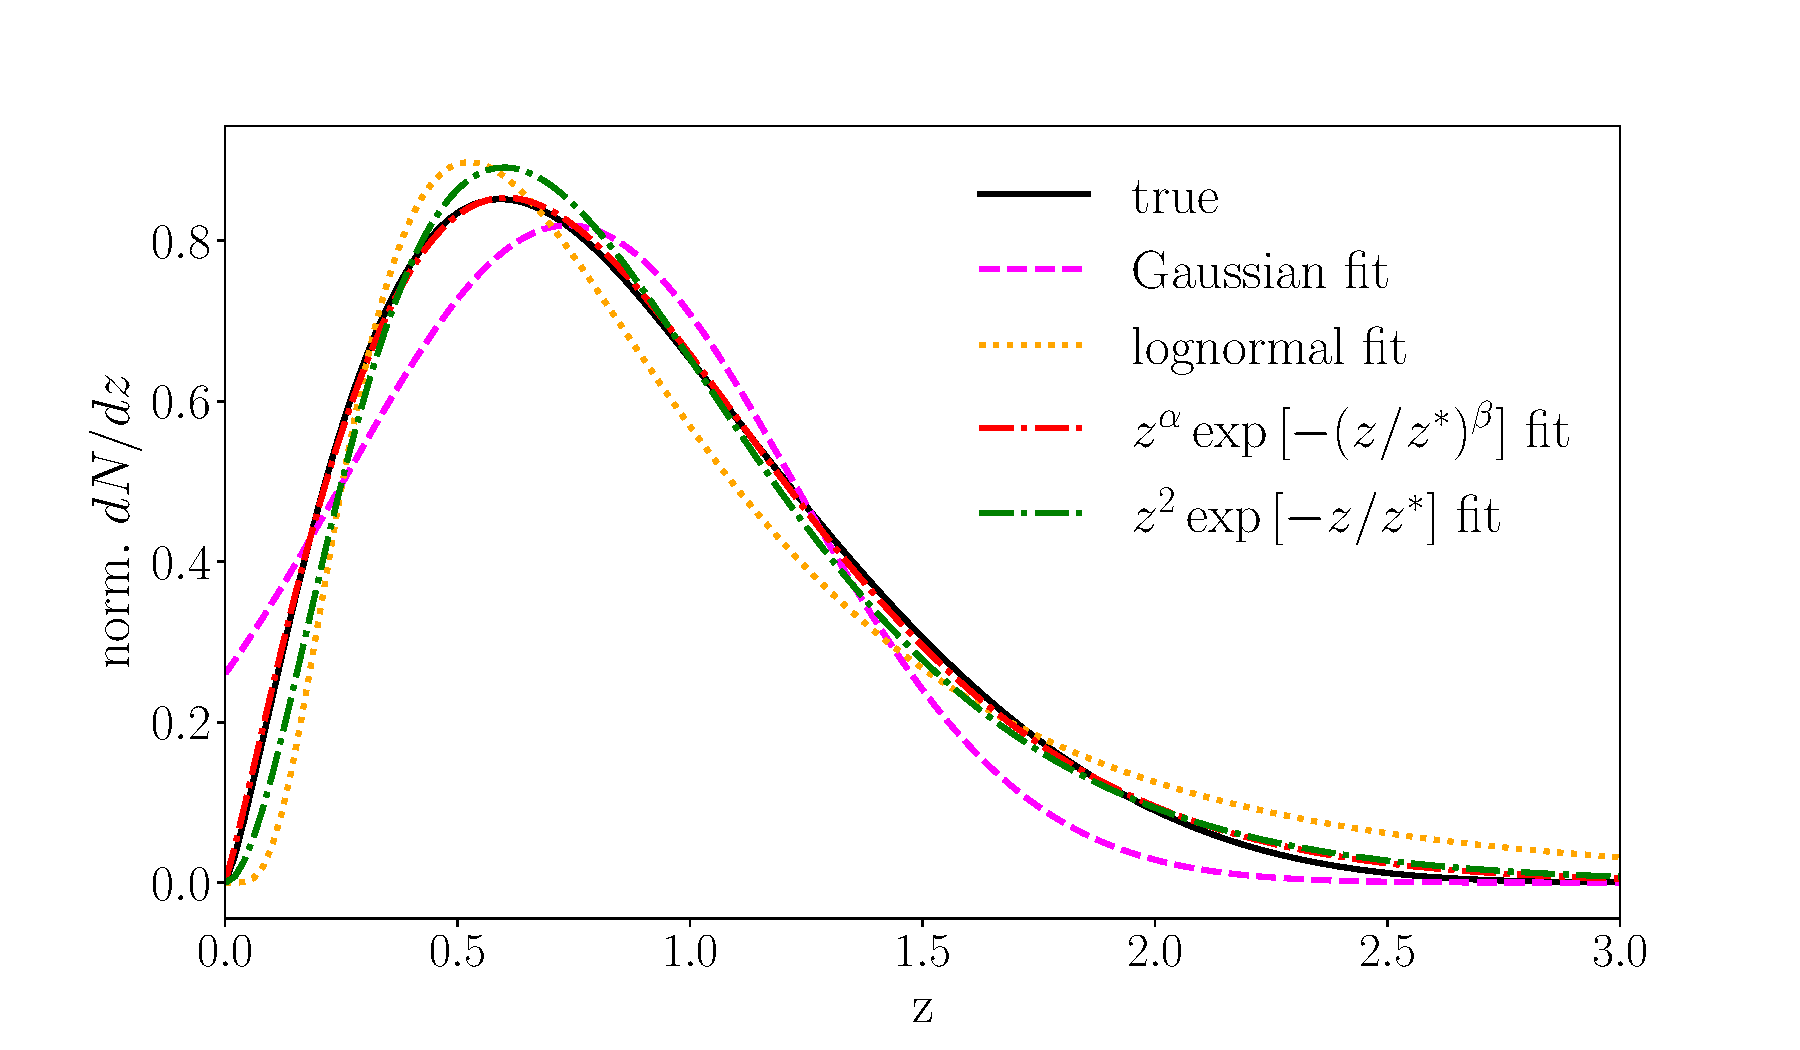
\includegraphics[width=1.0\columnwidth]{GaussVSlognorm_fit_dndz.pdf}
\caption{Different fitting functions were considered. The normalized `true' function here was taken from \cite{0004-637X-814-2-145} (solid black line), and the best fitting function is given in eq. \ref{eq:ngfit} (red dotted-dashed line).}
\label{fig:ngfits}
\end{figure}

% \begin{figure}
% \centering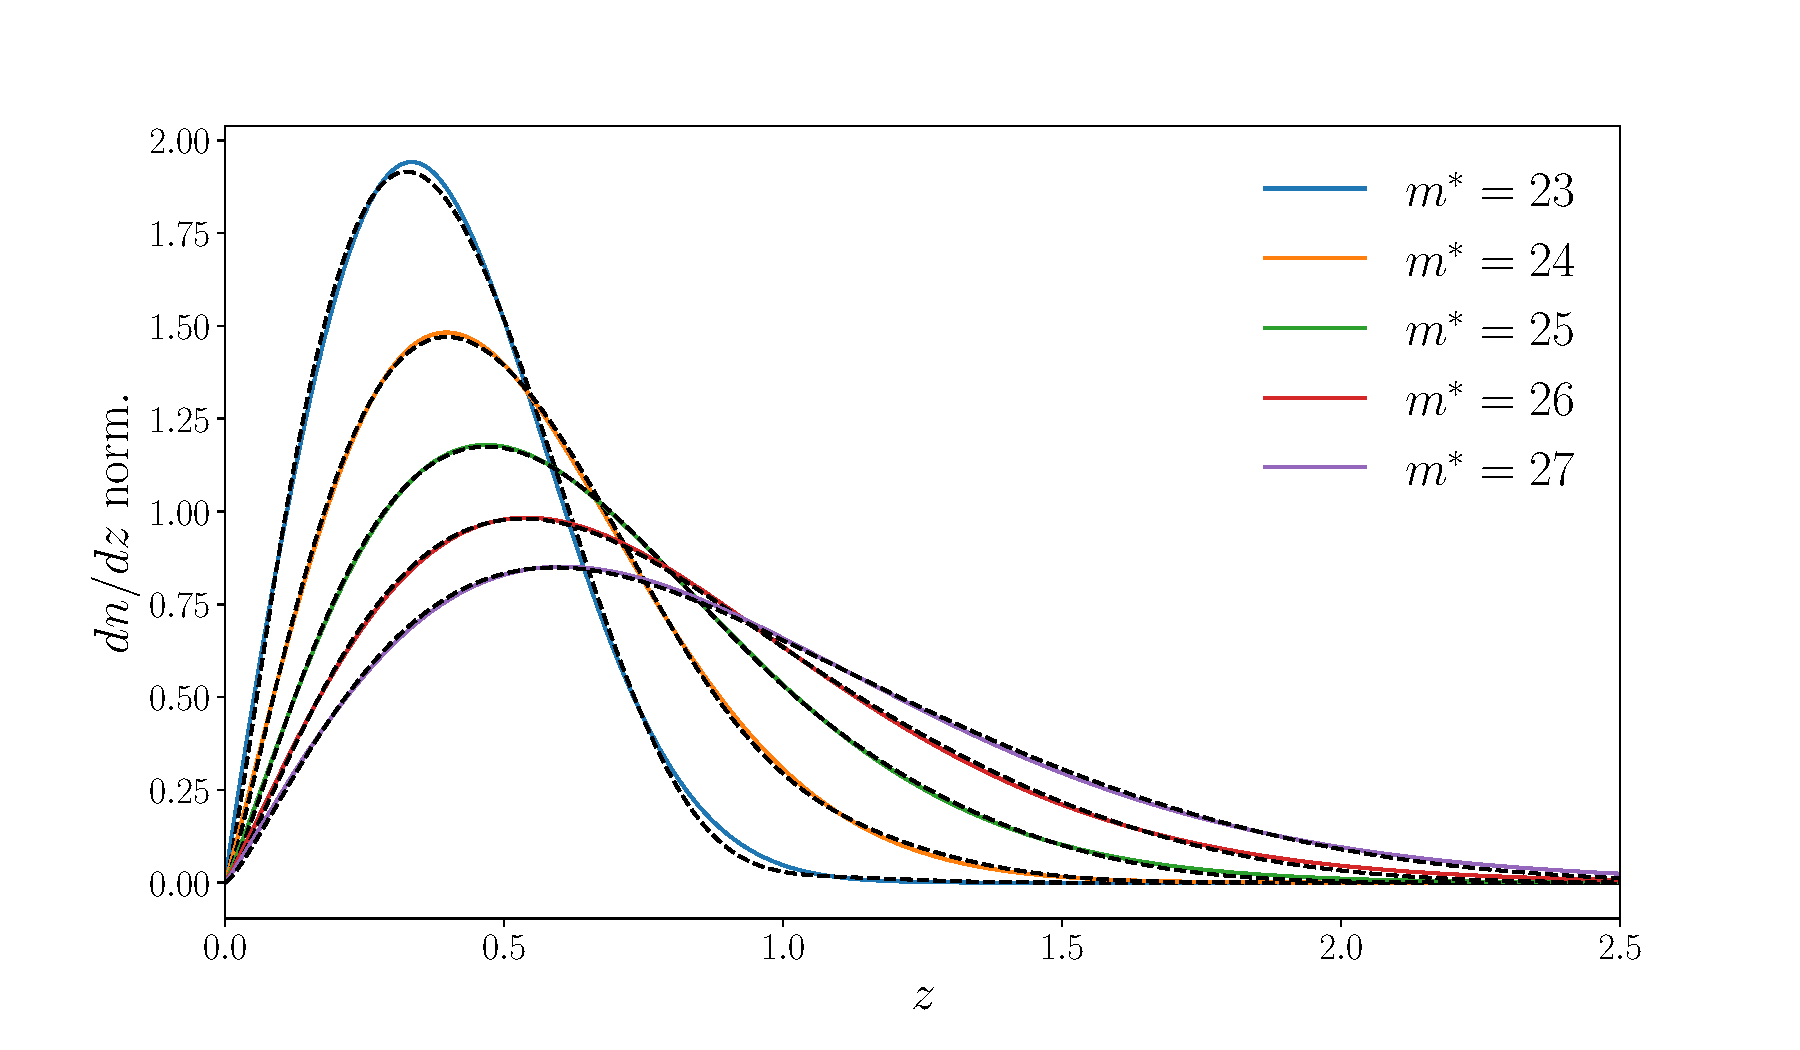
\includegraphics[width=.9\columnwidth]{dndz_fit_for_different_mag.pdf}
% \caption{We used a fit (solid lines, from eq. \ref{eq:ngfit}) of the galaxy number density function provided in \cite{0004-637X-814-2-145} (dashed black lines), in order to speed up numerical integration.}
% \label{fig:ngfitquality}
% \end{figure}

\begin{figure}
\centering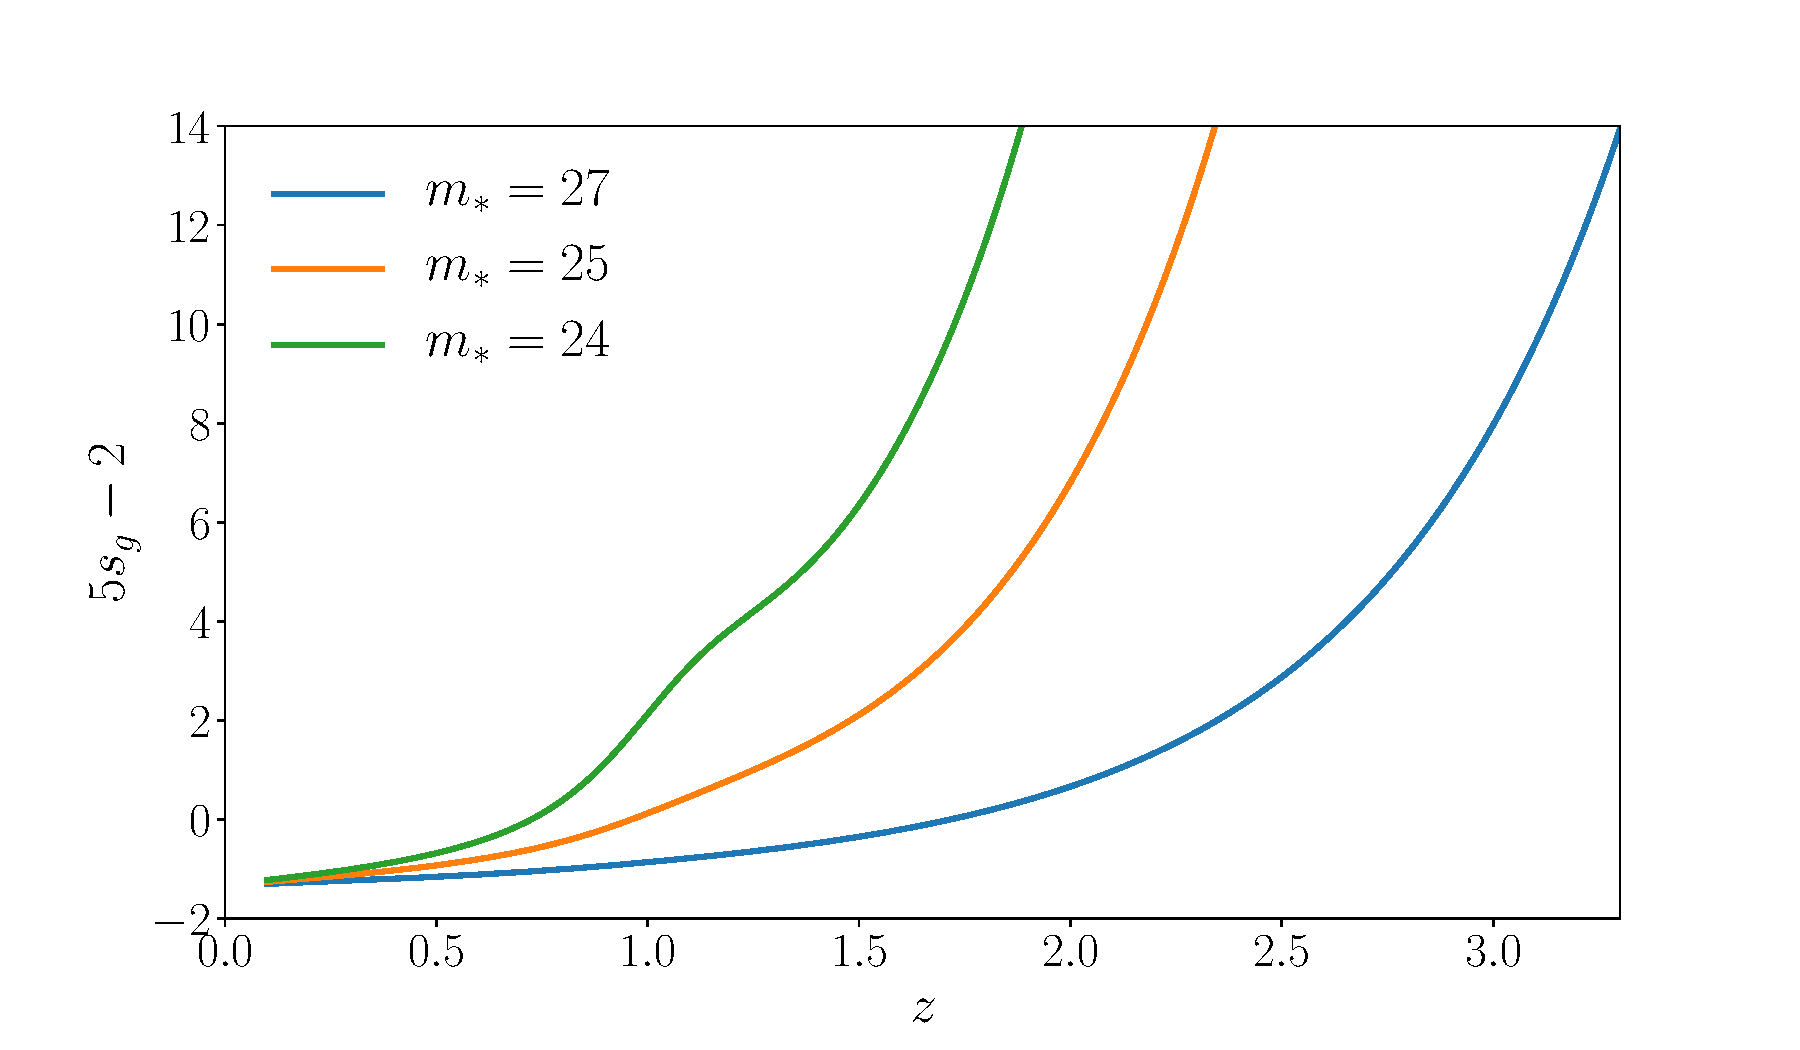
\includegraphics[width=0.85\columnwidth]{alpha.pdf}
\caption{The number count slope $s_g$ for different magnitude cutoff values. The maximum magnitude detectable with LSST is assumed to be $27$. Imposing a lower magnitude cutoff increases the shot noise, but also the number count slope, which increases the magnification signal. }
\label{fig:sg}
\end{figure}

\begin{figure}
\centering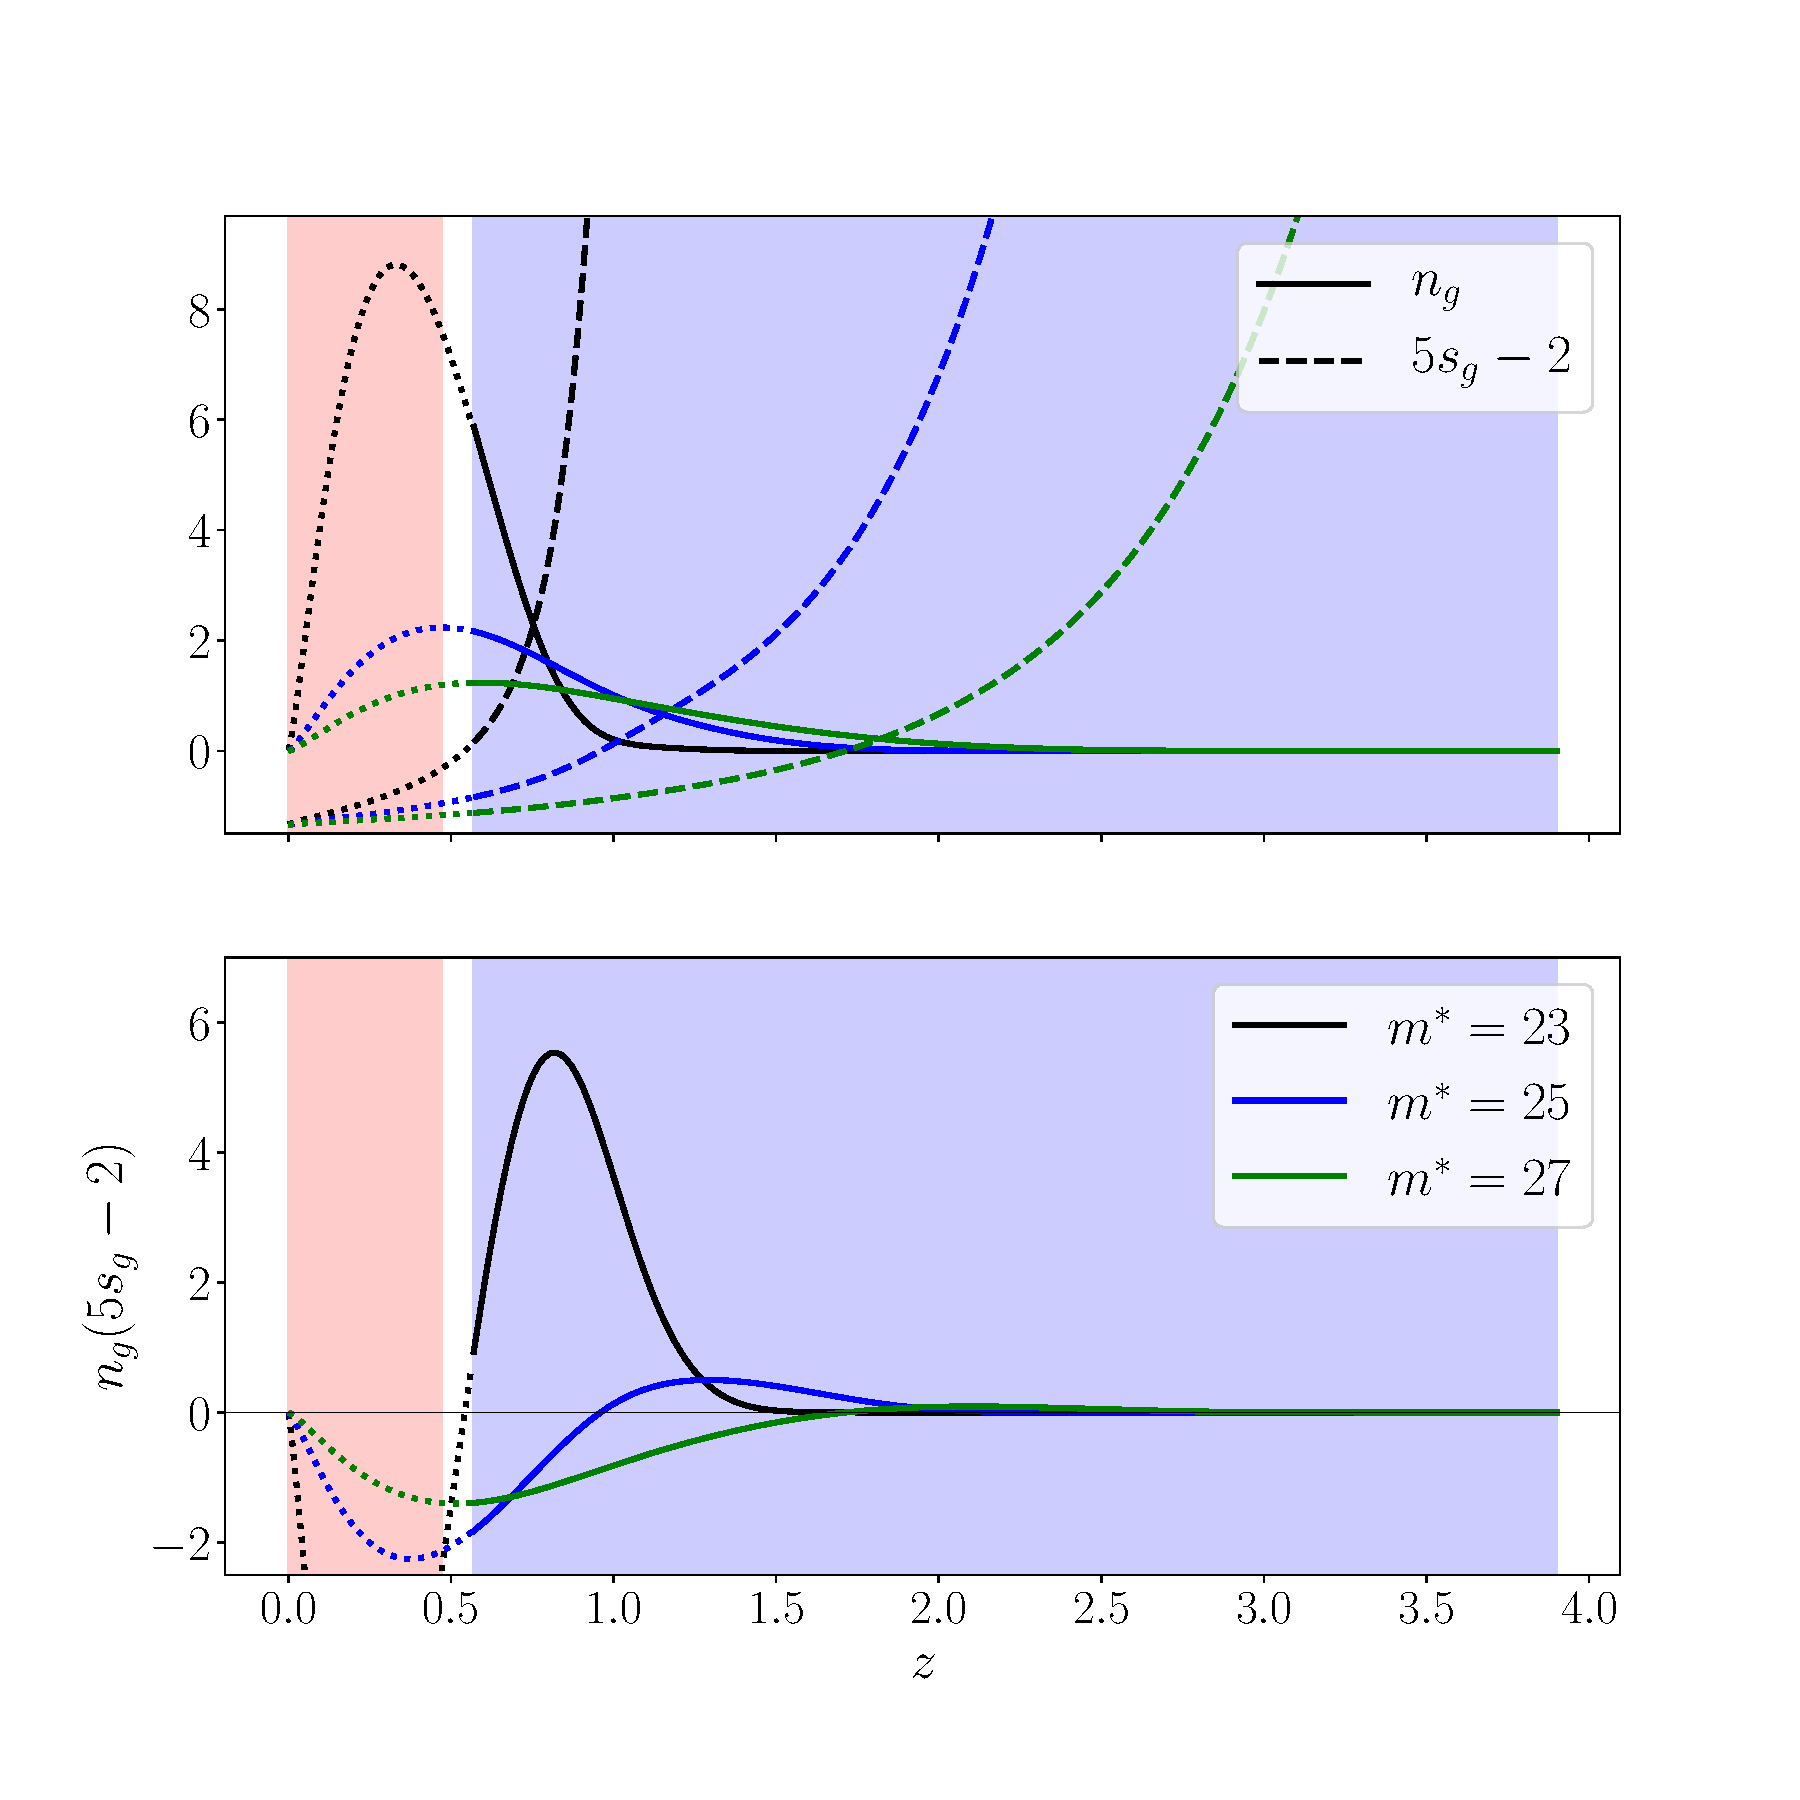
\includegraphics[width=0.95\columnwidth]{W_and_sg_SKAB2.pdf}
\caption{We illustrate the behavior of the lensing kernel with respect to the magnitude threshold $m^*$, using band 2 of SKA as an example. The red (blue) shaded areas indicate the foreground (background) redshift range. The upper panel displays the galaxy number density $n_{\rm g}$ (normalized to integrate to one inside the background bin), and the contribution of the number count slope $s_{\rm g}$. The bottom panel shows their product. The only term inside the integral eq. \ref{eq:gkernel} to potentially be negative is $5s_{\rm g} -2$. This demagnification leads to cancellation in the integration and thus to a smaller lensing signal. An appropriate magnitude cutoff enforces $5s_{\rm g} >2$ in the background redshift bin and thus improves the signal. However, this comes at the cost of increasing the galaxy shot noise.}
\label{fig:gkernel}
\end{figure}

\begin{figure}
\centering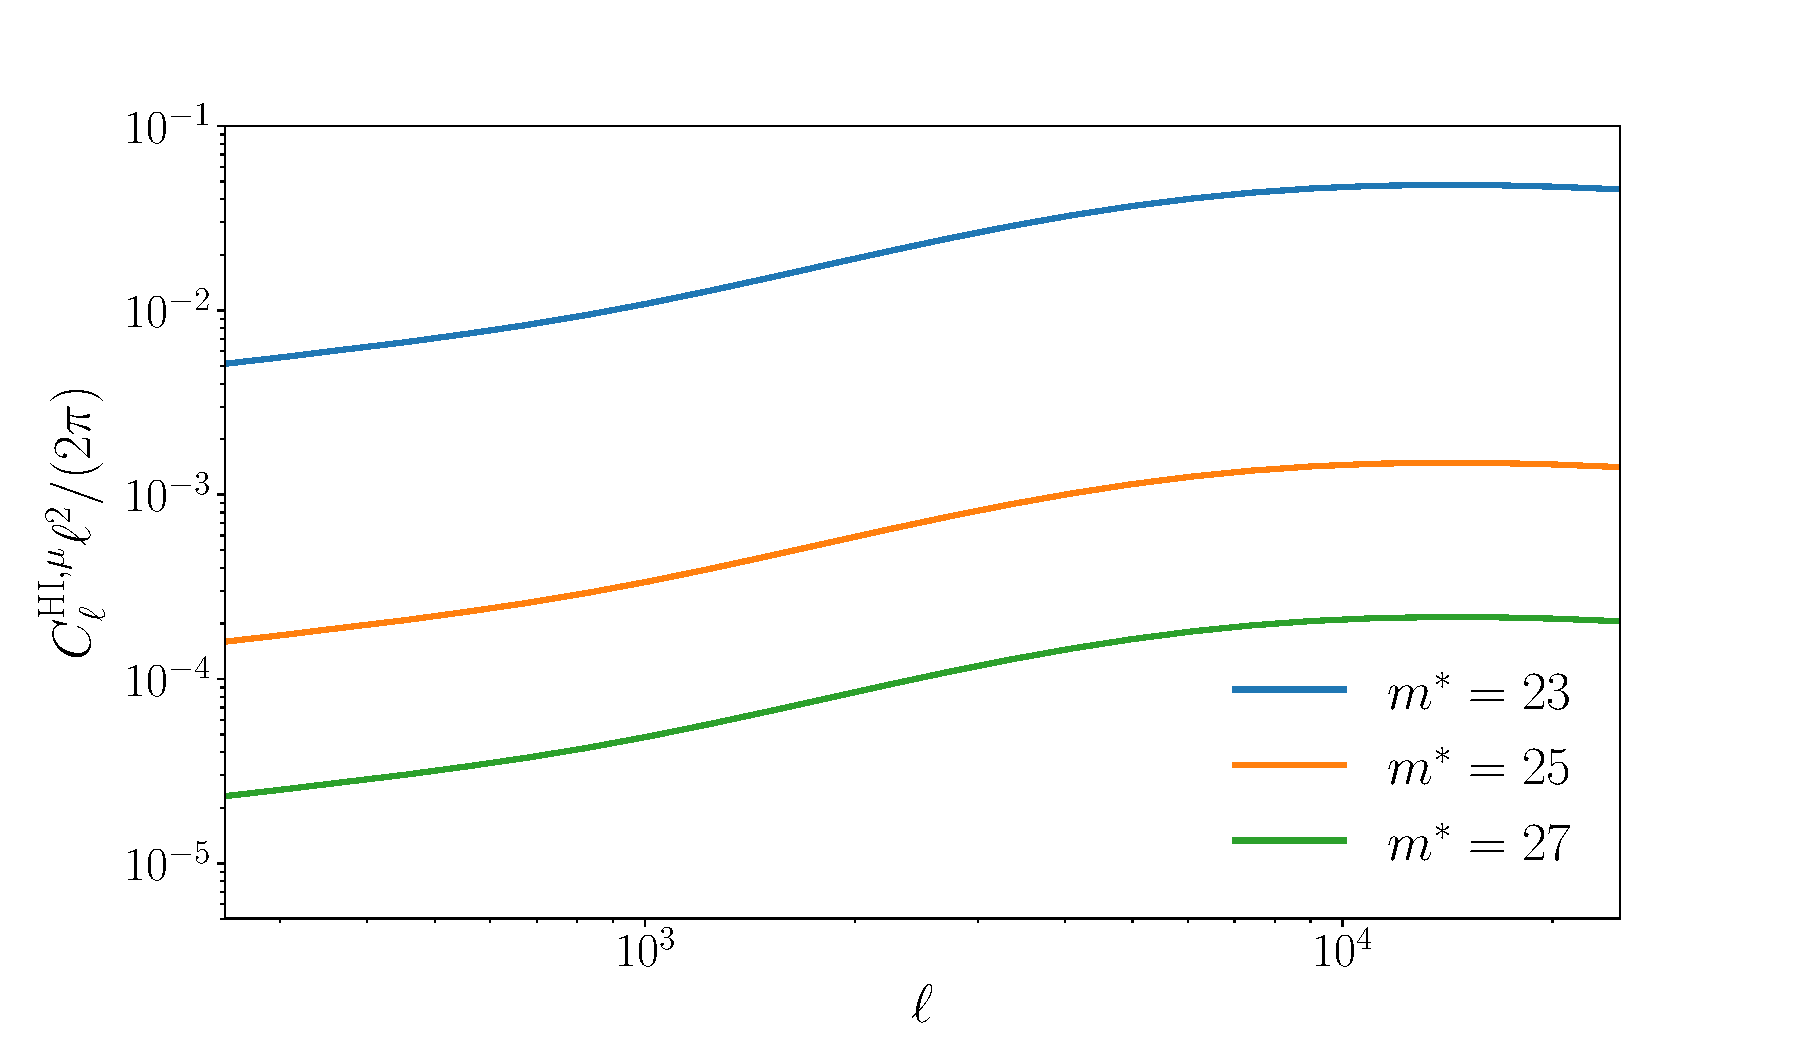
\includegraphics[width=.9\columnwidth]{HIxmag_Cls.pdf}
\caption{The HI-magnification cross-correlation power spectrum for a foreground redshift from $z=0.5$ to $1$ and background redshift from $z=1.5$ to $1.9$.}
\label{fig:HIxmag_Cls}
\end{figure}



The error in the measurement of the cross-correlation power spectrum is
\be
\label{eq:magerr}
\Delta C^{{\rm HI} - \mu}_\ell = \sqrt{\frac{2((C^{{\rm HI} - \mu}_\ell)^2+(C^{\rm gg}_\ell+C^{\rm shot})(C^{\rm HI-HI}_\ell+N_\ell))}{(2\ell+1)\Delta \ell f_{\rm sky}}} \, ,
\ee where $C^{\rm shot}$ the galaxy shot noise power spectrum, $N_{\rm \ell}$ the thermal noise of the intensity mapping instrument, $\Delta \ell$ the binning in multipole space, and $f_{\rm sky}$ the fraction of sky area overlap of both surveys. The auto-correlation power spectra are calculated as
\begin{equation}
C_\ell^{\rm HI-HI} = \frac{H_0}{c} \int dz E \biggl( \frac{ b_{\rm HI}\bar{T}_{21}(z) W(z) D}{r}\biggr)^2 P_{\rm cdm} \biggl( \frac{\ell + 1/2}{r} \biggr),
\end{equation}
and
\begin{equation}
  \label{eq:clgal}
C_\ell^{{\rm g-g}} = \frac{H_0}{cN_{\rm g}^2} \int dz E \biggl( \frac{ b_{\rm g }(z) n_{\rm g}(z) D}{r}\biggr)^2 P_{\rm cdm} \biggl( \frac{\ell + 1/2}{r} \biggr),
\end{equation}
with the galaxy bias $b_{\rm g}$ and HI bias $b_{\rm HI}$ given by fits to the results from \cite{0004-637X-814-2-145}:
\begin{equation}
  b_{\rm HI}(z) = 0.67 + 0.18 z + 0.05 z^2,{\rm~and}
\end{equation}

\begin{equation}
  b_{\rm g}(z) = 1+0.84 z.
  \label{eq:mag_gbias}
\end{equation}

The mean observed HI brightness temperature is calculated using the fit provided in \cite{2017arXiv170906099S}, which is based on the results from \cite{2015aska.confE..19S}:
\be
\bar{T}_{21} = 0.0559+0.2324z-0.024 z^2.
\ee


Equation \ref{eq:mag_gbias} is simplified, as the galaxy bias $b_{\rm g}$ should in principle depend on the magnitude cut $m^*$. We expect this to have a small effect on our results and ignore this dependence for now.

\section{Error calculations}

\subsection{HI intensity maps}
\ama{Pcdm}


We consider the experiments HIRAX and SKA1 MID to map the distribution of foreground HI. Together with the shot noise from LSST, their instrumental noise contributes to the error given by equation \ref{eq:magerr}.

HIRAX is a planned radio interferometer of $6$ m diameter dishes, sharing the site in the Karoo in South Africa with MeerKAT. We assume the full planned array of 1024 and the reduced set of 512 dishes, arranged in a dense square grid with $1$ m space between individual antennas. HIRAX' survey area is assumed to be $15.000$ deg${}^2$ and the integration time is taken to be two full years (corresponding to 4 years observation). It uses full cross-correlation and we assume a constant system temperature of 50 K on its entire frequency coverage ranging from $400$ to $800$ MHz \citep{2016SPIE.9906E..5XN}.


At the same time, SKA1 is assumed to have only one year worth of integration time but a larger survey area of 16900 deg${}^2$ (this corresponds to the maximum possible survey overlap with LSST). SKA1 MID will consist of different dish types: the 64 MeerKAT dishes with $13.5$ m and $133$ SKA dishes of $15$ m diameter. For simplicity, we assume all dishes to be identical, with the average dish diameter $\tilde{D}_\mathrm{dish} = (64*13.5 + 133*15)/(64+133)$ and use a Gaussian beam pattern. We consider two observational bands: band 1 ranging from $350$ to $1050$ MHz, and band 2 from $950$ to $1750$ MHz. The system temperature is assumed a constant $30$ K over the entire frequency range. This is conservative on low redshifts. For high-redshift foreground bins, the system temperature increases beyond that, but at the same time the galaxy shot noise becomes the dominant source of error and magnification detections quickly become extremely difficult for foregrounds with $z \gtrsim xxx$ \ama{finalize}. This justifies our assumption of constant system temperature for both SKA and HIRAX. For both experiments, we use equally spaced redshift bins of width $dz = 0.5$ \ama{finalized at the end} . A more realistic treatment would have to take into account the frequency dependence of the noise temperatures of both experiments, and the different dish and receiver types of SKA1. However, we expect this to only have a small effect on our results.


Following \cite{0004-637X-803-1-21} for the intensity mapping noise calculations, we calculate the single dish noise for SKA as
\begin{equation}
  N^{\rm SD}_\ell = \sigma_\mathrm{pix}^2\Omega_\mathrm{pix}W_\ell^{-1},
\end{equation}

with the solid angle per pixel $\Omega_\mathrm{pix} = 4\pi/N_\mathrm{pix}$, the number of pixels $N_\mathrm{pix}$, the beam smoothing function $W_\ell = \exp\bigl(-\ell^2 \Theta_\mathrm{FWHM}^2/(8\ln{2})\bigr)$, the pixel noise $\sigma_\mathrm{pix} = T_\mathrm{sys} * \sqrt{ N_\mathrm{pix} f_\mathrm{sky} / ( t_\mathrm{tot} \delta_\nu N_\mathrm{dish})}$ and the frequency resolution $\delta_\nu$.

For HIRAX, we calculate the interferometer noise
\begin{equation}
  N^{\rm i}_\ell = \frac{(\lambda^2 T_{\rm sys})^2}{2 A_{\rm e}^2 d\nu n(u) t_{\rm p}}
\end{equation}
with the frequency bin width $d\nu$, the time per pointing $t_{\rm p} = t_{\rm tot} / N_{\rm p}$, the effective collecting area of one dish $A_{\rm e} = (D_{\rm dish}/2)^2 \pi$, and using the relation $u = \ell / (2 \pi)$ for the baseline density $n(u)$.

For all experiments we assumed full survey overlap with LSST.
\subsection{Photometric galaxy counts}


The code from \cite{0004-637X-814-2-145} uses the Schechter luminosity function from \cite{2010MNRAS.402.1330G} to fit number counts from \cite{2013LRR....16....6A}:

\be 
\tilde{n}_{\rm g}(z, L>L_{\rm cut}) = \int_{x_{\rm cut}}^\infty \epsilon \phi^* x^\alpha \exp^{-x} dx,\, x\equiv L/L^*(z).\nonumber
\ee
\ama{explain all parts of this equation}

\ama{We can go without this, it will just run longer:}
In order to increase computational speed, we adapt the fit from \cite{2009arXiv0912.0201L} to approximate the result from \cite{0004-637X-814-2-145} for the LSST galaxy number density $n_{\rm g}$ as follows,
\be
n_{\rm g}(z) \propto z^\alpha \exp \bigl( -\bigl(\frac{z}{z^*}\bigr)^\beta \bigr),
\label{eq:ngfit}
\ee
where we optimize the parameters $\alpha$, $\beta$ and $z^*$ as functions of magnitude cutoff $m^*$ by interpolation. The overall amplitude is irrelevant in \ref{eq:gkernel} as $n_{\rm g}$ is normalized to integrate to one, but it is required to calculate the shot noise. For this we normalize the LSST sample to be a total of $\sim 6.3\times 10^9$ galaxies at best achievable $m^*$. See figure \ref{fig:ngfits} for a comparison of different fitting functions.

To calculate the galaxy shot noise, we use the expected number density of an LSST galaxy survey \citep{0004-637X-814-2-145} to normalize the integral of the fitting function (eq. \ref{eq:ngfit}) at $m^* = 27$ over the full redshift range. 


The galaxy shot noise for LSST is calculated as $C^\mathrm{shot} = 4\pi/N^{\rm LSST}(z)$, with $N^{\rm LSST}_i$ the number of detected galaxies in the considered redshift bin i. We consider all LSST redshift bins having their upper edge at $z_{\rm max}^{\rm LSST} = 3.9$, and the lower bin edge at a small separation from the upper edge of the foreground bin, $z^{\rm fg}_i + 0.1$. The choice of a separation of $\Delta z = 0.1$ is conservative, ruling out any cross-correlations from possible overlaps, caused for example by the uncertainty in the photometric redshift measurements of LSST. We calculate the number count slope for LSST using an adjusted version of the code provided in \cite{0004-637X-814-2-145} to extend to more stringend luminosity cutoffs $m^*$. It exploits \ref{eq:ngNg} to calculate \ref{eq:sg} more efficiently.
We then interpolate $(5s_{\rm g}-2)n_{\rm g}$ on a fine grid ($z$ and $m^*$) to speed up calculations.


The theoretical prediction for the observable magnification signal is given in figure \ref{fig:HIxmag_Cls}, with its amplitude being proportional to a redshift integral of the number count slope $s_g$ (eq. \ref{eq:sg}, \ref{eq:clhimu}; fig. \ref{fig:sg}). The number count slope, and thus the signal amplitude, can be increased by adjusting the magnitude cutoff $m^*$ of the galaxy survey at the cost of increasing the shot noise.


In order to illustrate the different error contributions, we define the following quantities:
\begin{align}
\Delta C_\ell^{\rm HI-HI} &= \sqrt{\frac{2}{(2\ell+1)\Delta\ell f_{\rm sky}}} \bigl( C_\ell^{\rm HI-HI} + N_\ell \bigr)& \nonumber \\ &\equiv \Delta_{\rm CV}^{\rm HI-HI} + \Delta_{N_\ell}^{\rm HI-HI},&
\label{eq:deltah-h}
\end{align}

\be
\Delta C_\ell^{\rm g-g} = \sqrt{\frac{2}{(2\ell+1)\Delta\ell f_{\rm sky}}} \bigl( C_\ell^{\rm g-g}+ C^{\rm shot} \bigr) \equiv \Delta_{\rm CV}^{\rm g-g} + \Delta_{\rm shot}^{\rm g-g},
\label{eq:deltag-g}
\ee

and


\begin{align}
  (\Delta C_\ell^{{\rm HI-}\mu})^2 = \frac{2}{ (2\ell+1)\Delta\ell f_{\rm sky}} \biggl(   ((C_\ell^{{\rm HI-}\mu})^2  + C_\ell^{\rm g-g}C_\ell^{\rm HI-HI} ) \nonumber \\
  + ( C^{\rm shot}C_\ell^{\rm HI-HI} + N_\ell C_\ell^{\rm g-g} +  C^{\rm shot}N_\ell)  \biggr).
  \label{eq:deltah-mu}
\end{align}

Here we grouped together all terms containing noise in $\Delta^{{\rm HI-}\mu}_{{\rm shot,~}N_\ell}$, $\Delta_{\rm shot}^{\rm g-g}$ and $\Delta_{N_\ell}^{\rm HI-HI}$. All remaining terms are noise-free, proportional to the power spectra and correspond to the contribution of cosmic variance: $\Delta^{{\rm HI-}\mu}_{\rm CV}$, $\Delta_{\rm CV}^{\rm g-g}$ and $\Delta_{\rm CV}^{\rm HI-HI}$.


The multipole resolution is set by the maximum scale accessible by the SKA, i.e. the survey area $S_{\rm area}$. We estimate $\ell_{\rm min}^{\rm SKA} = 2\pi/\sqrt{S_{\rm area}} \sim 3$. For the interferometer HIRAX it is set by the field of view ($\rm fov$) which depends on frequency. For the sake of simplicity we ignore this dependence and assume a mean ${\rm fov} = 35.5 {\rm~deg}^2$ \citep{2016SPIE.9906E..5XN}, giving $\ell_{\rm min}^{\rm HIRAX} = 2\pi/\sqrt{\rm fov} \sim 60$. From the signal to noise ratio $C_\ell^{{\rm HI} - \mu} / \Delta C^{{\rm HI} - \mu}_\ell$ we calculate the cumulative signal to noise as

\be
{\rm S2N}_\ell = \sqrt{\sum_{\bar{\ell}=\ell_{\rm min}}^\ell (C_{\bar{\ell}}^{{\rm HI} - \mu} / \Delta C^{{\rm HI} - \mu}_{\bar{\ell}})^2},
\label{eq:s2ncum}
\ee
where the sum runs over the relevant $\ell$ values, with the minimum and resolution set by $\ell_{\rm min}$.

\section{Results}


\ama{Include also a table!}


\begin{figure}
\centering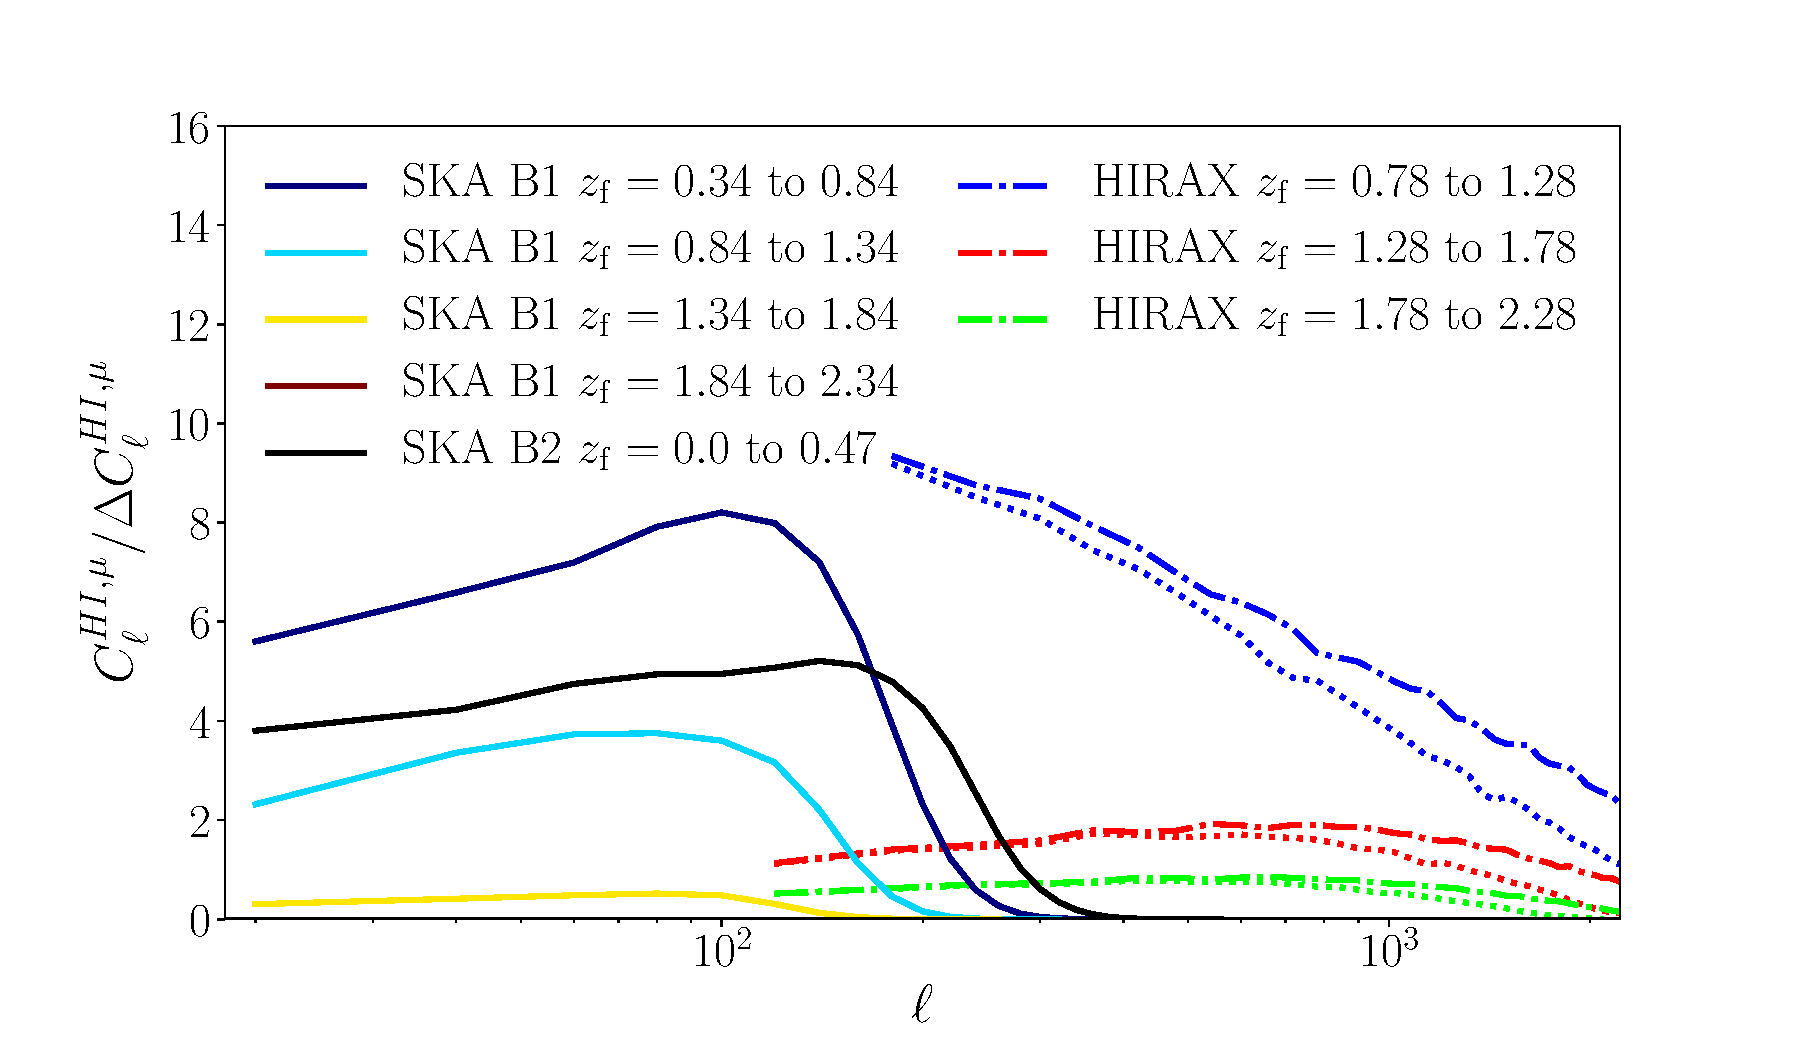
\includegraphics[width=.99\columnwidth]{S2N_SKA_HIRAX.pdf}
\centering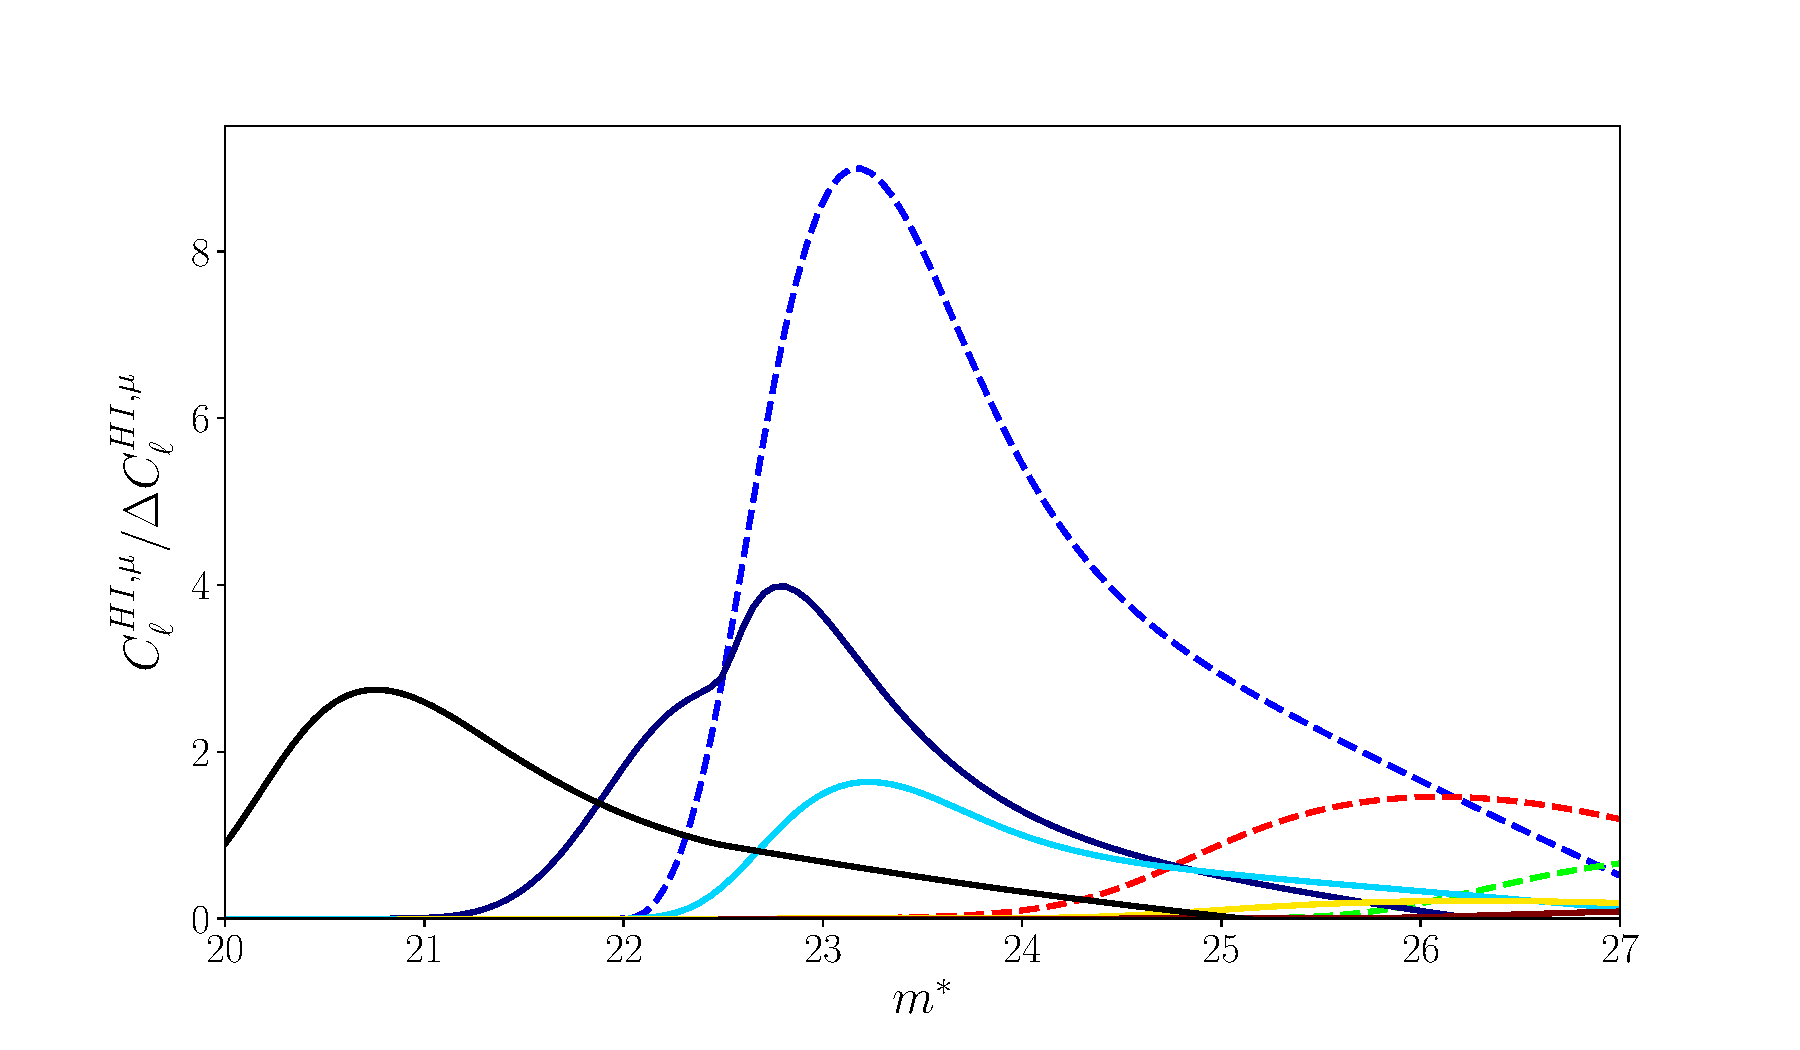
\includegraphics[width=0.99\columnwidth]{S2N_of_mstar.pdf}
\captionsetup{width=0.95\linewidth}
\caption{{\sl Upper panel:} The expected signal to noise ratio of the magnification signal for the combinations HIRAX 1024 (dotted-dashed lines), HIRAX 512 (dotted lines) and SKA1 (dashed lines) with LSST. We use different foreground redshift bins, always combined with one single non-overlapping background bin. The gray shaded area indicates the start of nonlinear regime, which depends on redshift. On smaller scales shot noise dominates, therefore the $512$ dish version of HIRAX performs surprisingly well compared to the full array with $1024$ dishes.
{\sl Lower panel:} The optimization of the signal to noise ratio as a function of magnitude cutoff $m^*$. For SKA $\ell = 80$ and for HIRAX $\ell = 200$.}
\captionsetup{width=.9\linewidth}
\label{fig:S2N}
\label{fig:S2Nmstar}
\end{figure}

% \begin{figure}
% \centering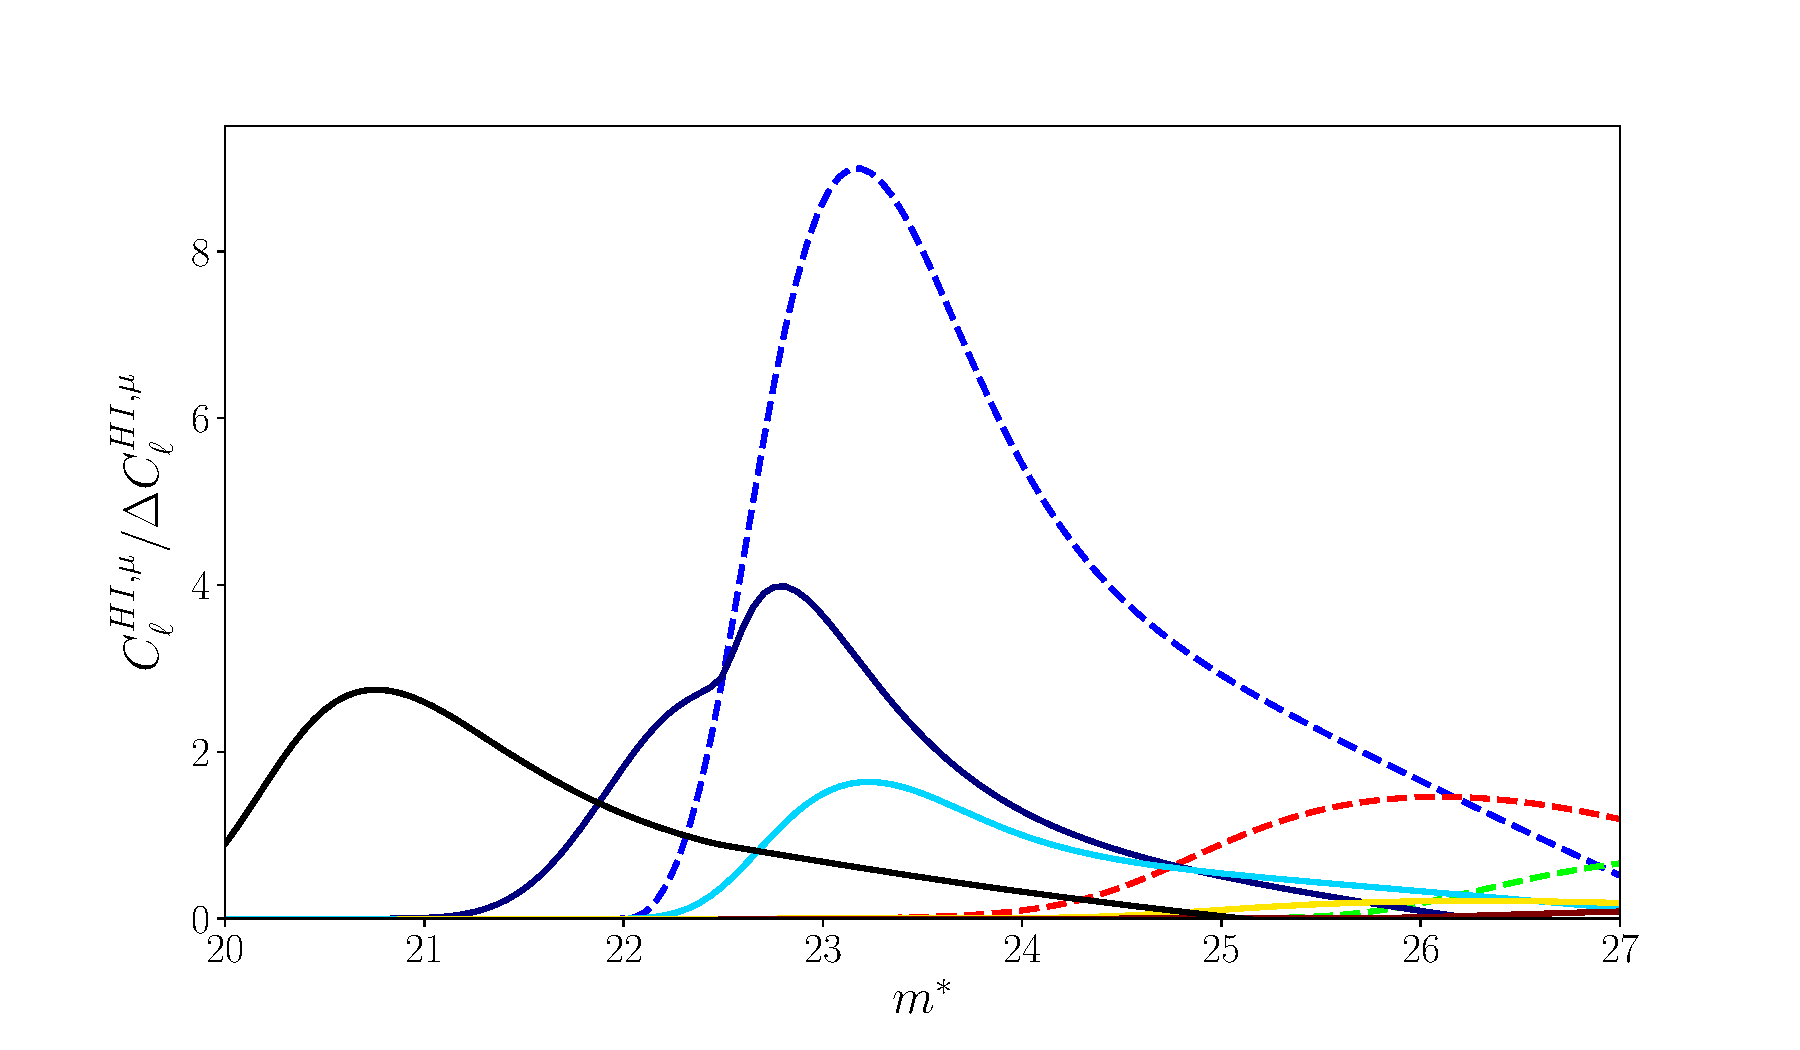
\includegraphics[width=0.8\columnwidth]{S2N_of_mstar.pdf}
% \caption{Colors and lines as in fig. \ref{fig:S2N}, here showing the optimization of the signal to noise ratio as a function of magnitude cutoff $m^*$. For SKA $\ell = 80$ and for HIRAX $\ell = 200$.}
% \label{fig:S2Nmstar}
% \end{figure}

\begin{figure}
\centering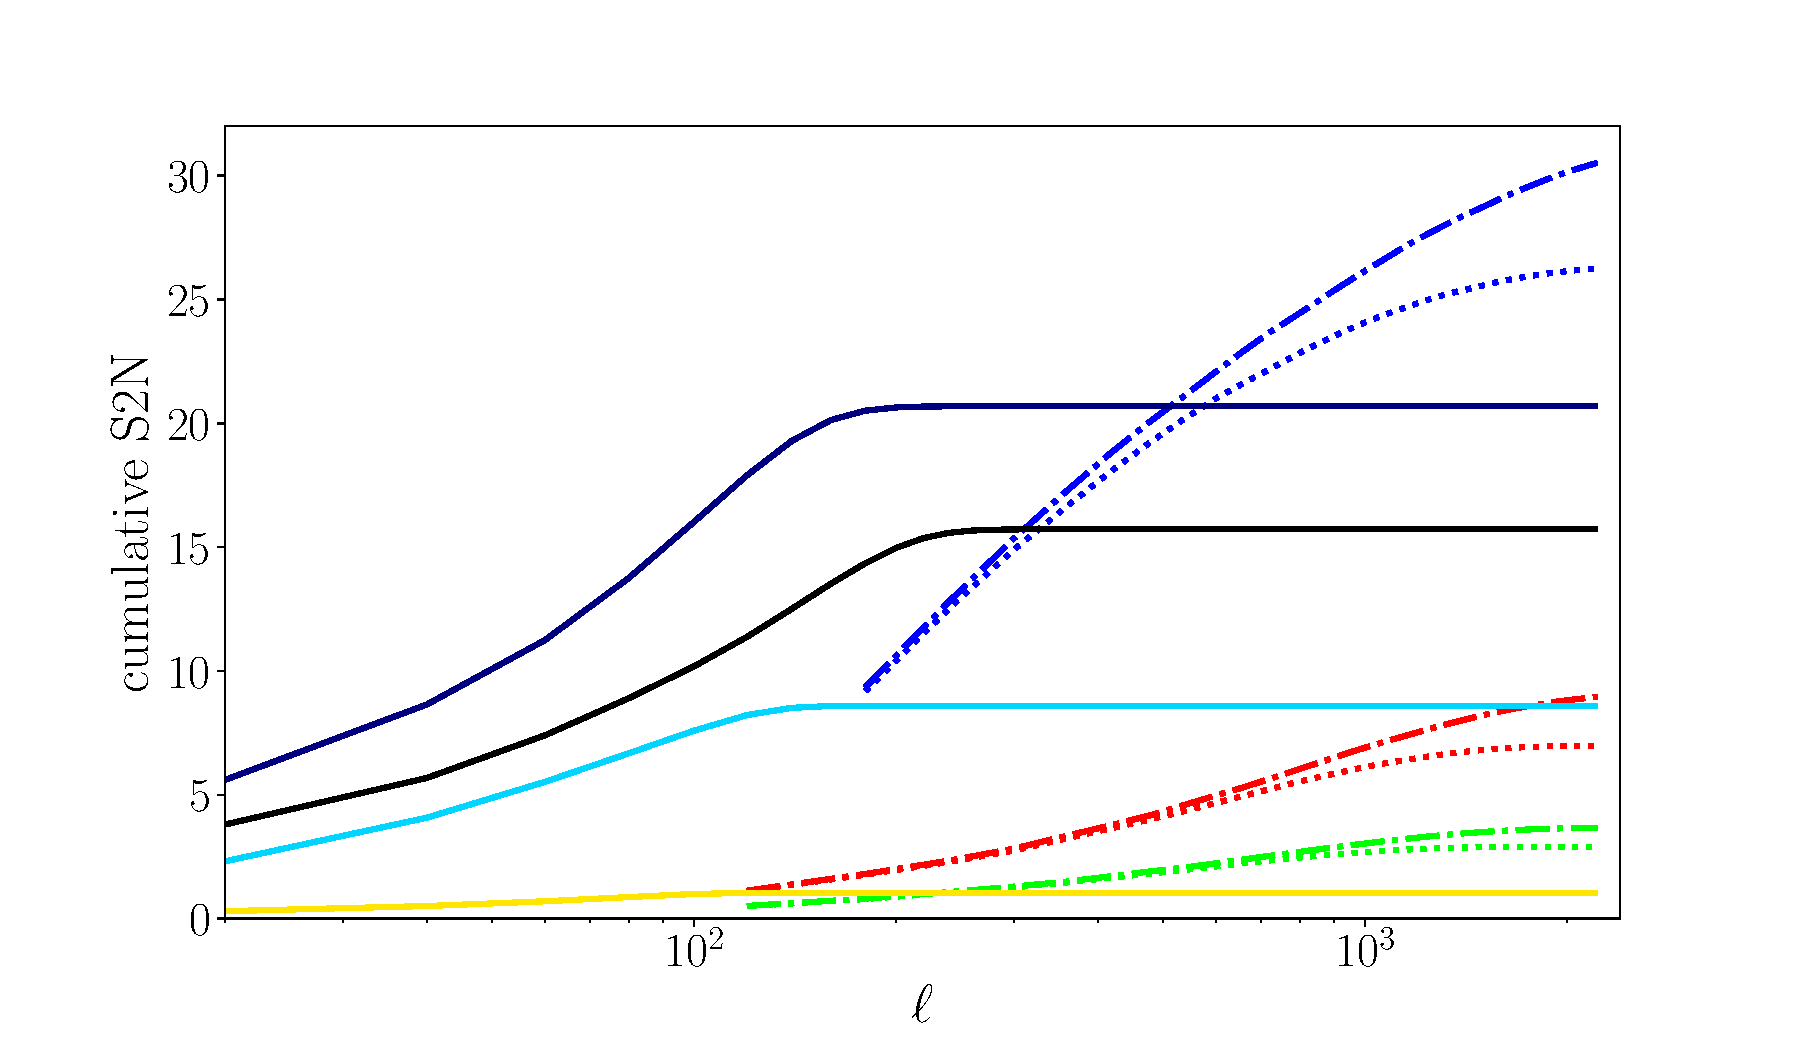
\includegraphics[width=.99\columnwidth]{S2N_SKA_HIRAX_CUM.pdf}
\centering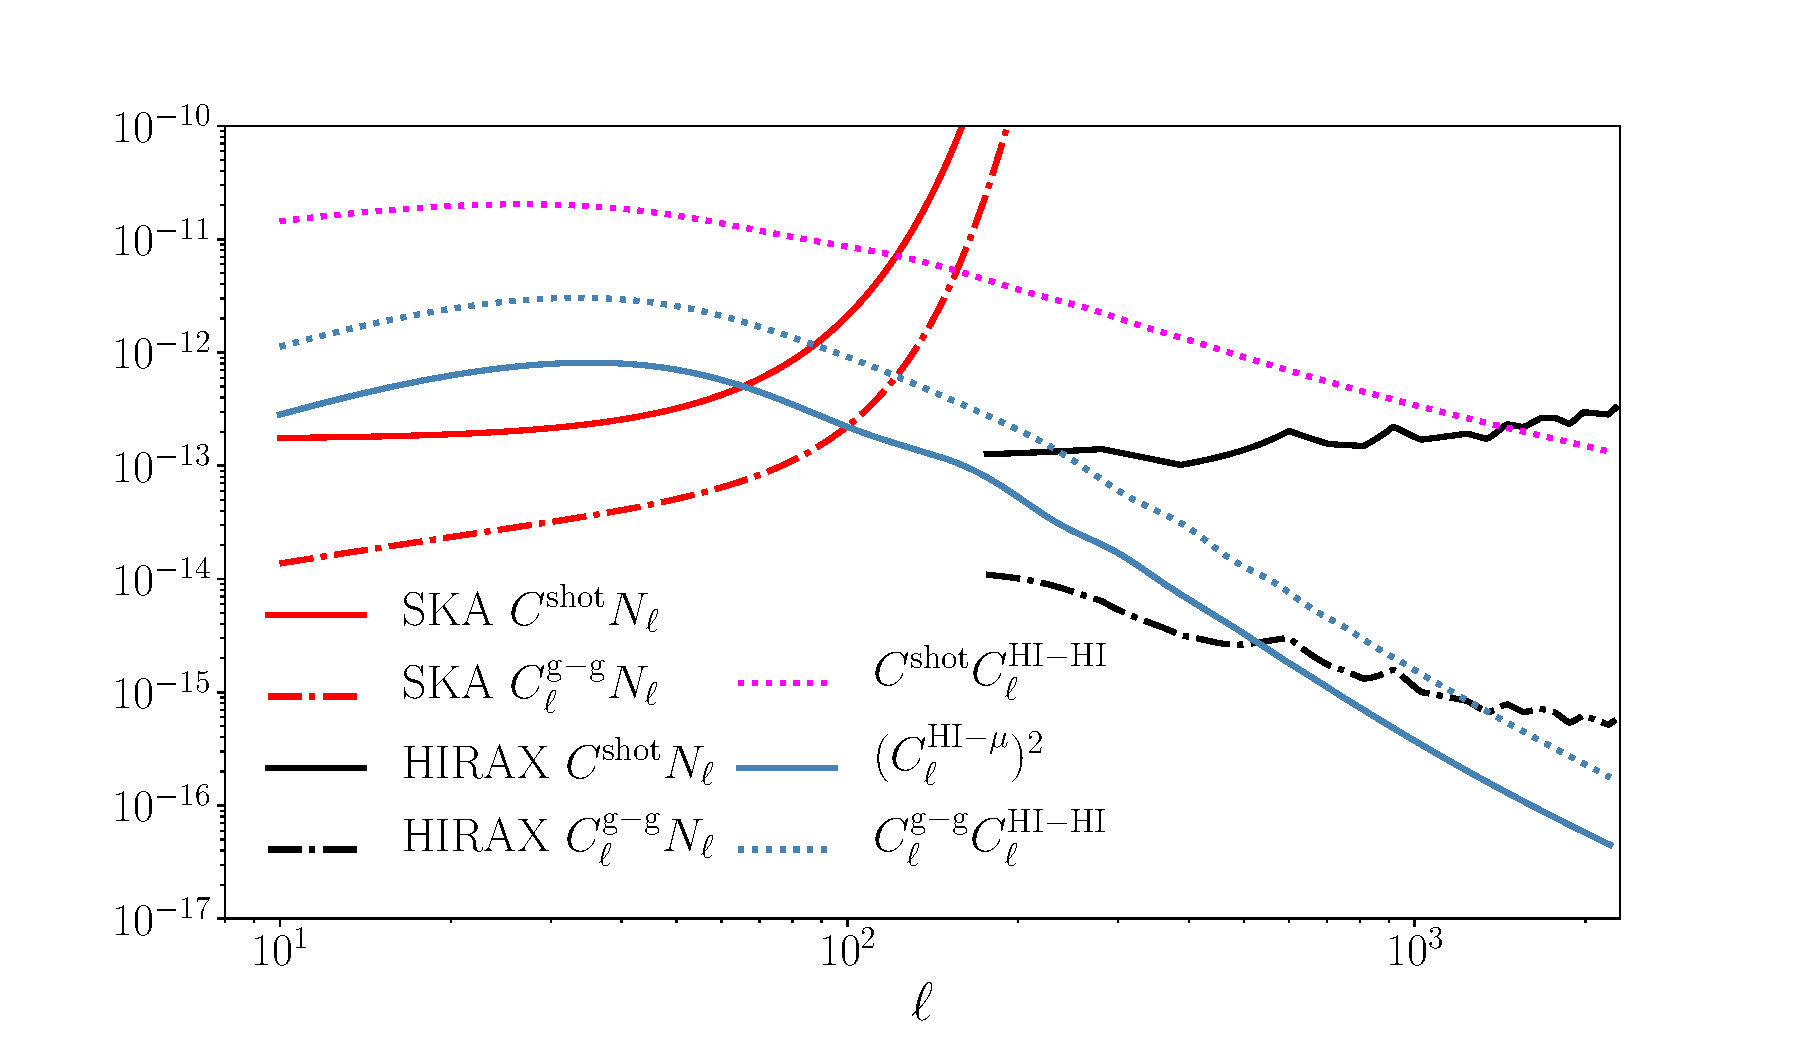
\includegraphics[width=.99\columnwidth]{X_error_contributions.pdf}
\captionsetup{width=.9\linewidth}

\caption{{\sl Upper panel:} Similar to fig. \ref{fig:S2N} but showing the cumulative signal to noise ratio instead (eq. \ref{eq:s2ncum}). For HIRAX especially, the error is dominated by the galaxy shot noise. Therefore even the down-scaled design with $512$ dishes yields very similar results compared to the full proposal with $1024$ dishes. SKA clearly outperforms HIRAX due to its much better multipole resolution of $\ell_{\rm min}^{\rm SKA} = 3$.
{\sl Lower panel:} All contributions to $\Delta C_\ell^{\mathrm{HI-}\mu}$ as in eq. \ref{eq:deltah-mu}, for a foreground redshift bin from $z=0.85$ to $1.35$ and a background bin $z\geq1.45$. Terms proportional to the SKA (HIRAX) noise are plotted in red (black). Terms proportional to hot noise and cosmic variance are plotted cyan and steel blue. For this choice of binning, the HI intensity mapping noise is subdominant, with shot noise the biggest source of instrumental noise, still dominated by cosmic variance \ama{confirm this statement}. Note that the choice of foreground and background redshift in this plot is only to ease comparison, but not ideal for magnification measurements.}
\label{fig:S2N_cum}
\label{fig:x_error_contributions}
\end{figure}


% \begin{figure}
% \centering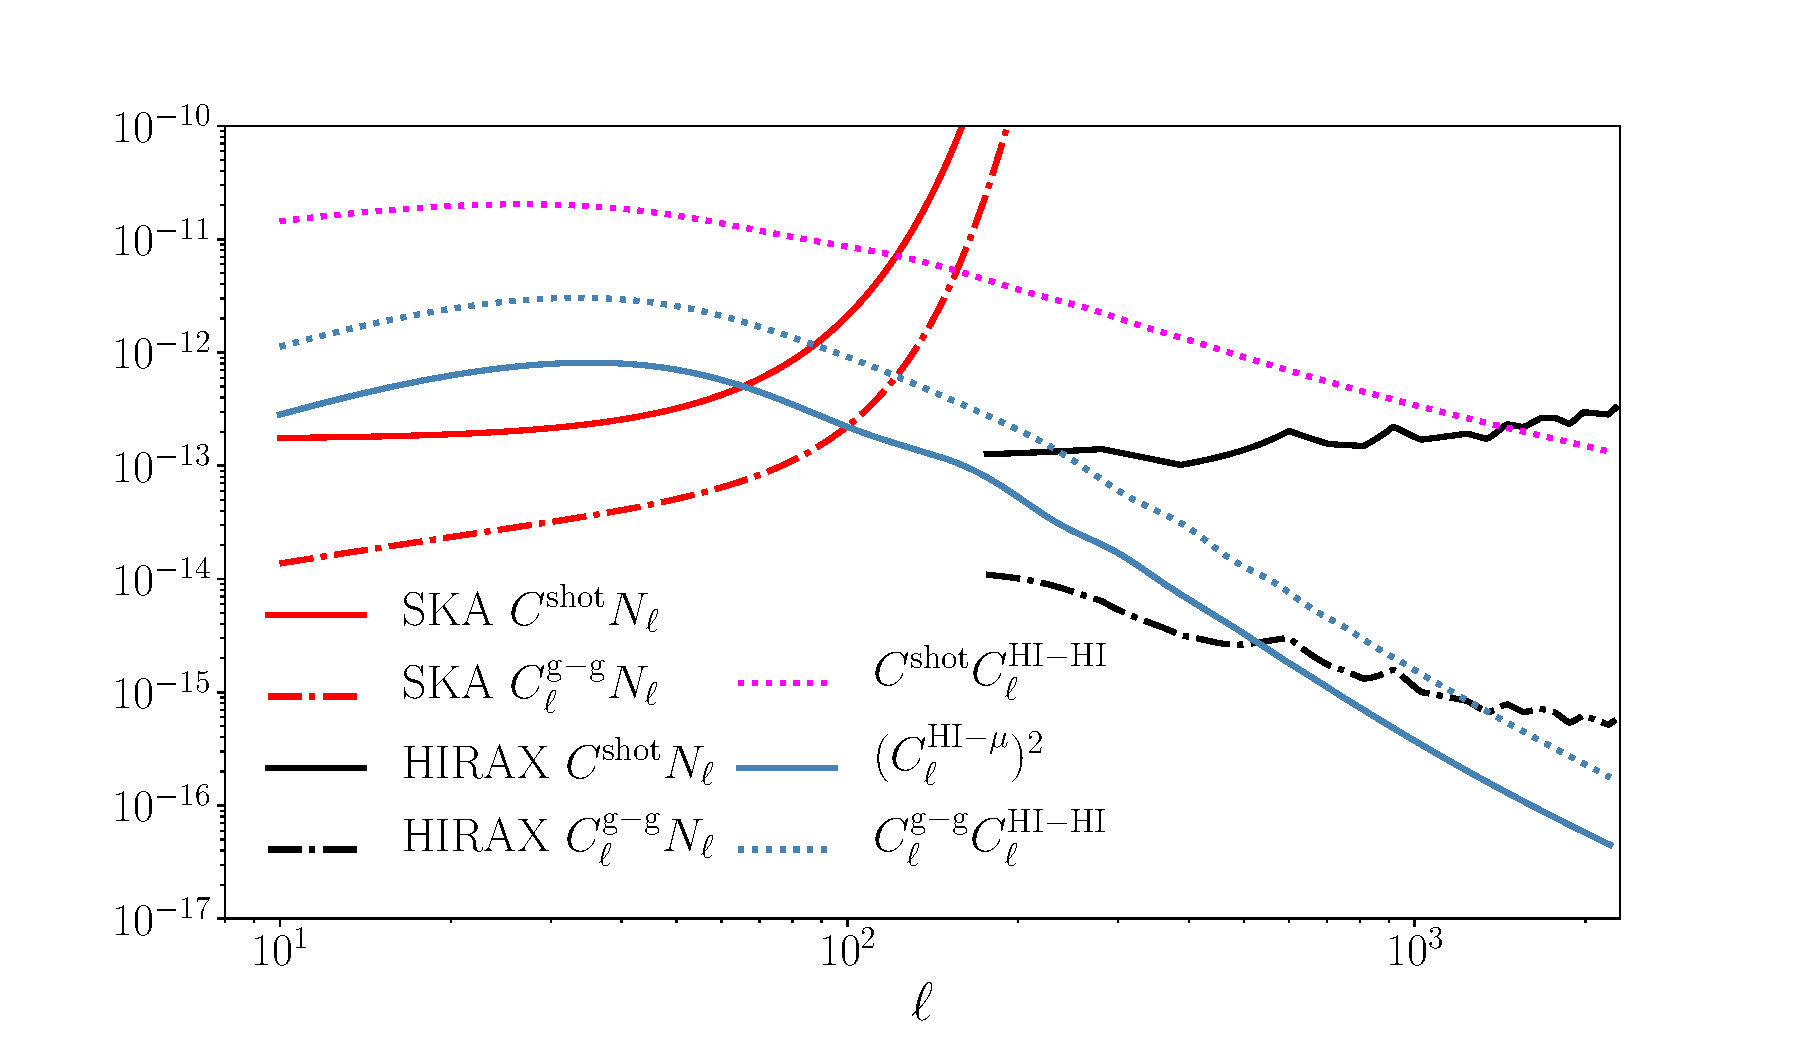
\includegraphics[width=.7\columnwidth]{X_error_contributions.pdf}
% \caption{Contributions to $\Delta C_\ell^{\mathrm{HI-}\mu}$ as defined in eq. \ref{eq:deltah-mu}, for a foreground redshift bin from $z=0.85$ to $1.35$ and a background bin $z\geq1.45$. Due to the different value of the optimal magnitude threshold for SKA and HIRAX, the expected signal amplitude slightly differs, so does the cosmic variance error. This difference is small and not shown in this plot. Note that the choice of foreground and background redshift in this plot is only to ease comparison, but not ideal for magnification measurements. }
% \label{fig:x_error_contributions}
% \end{figure}

% \begin{figure}
% \centering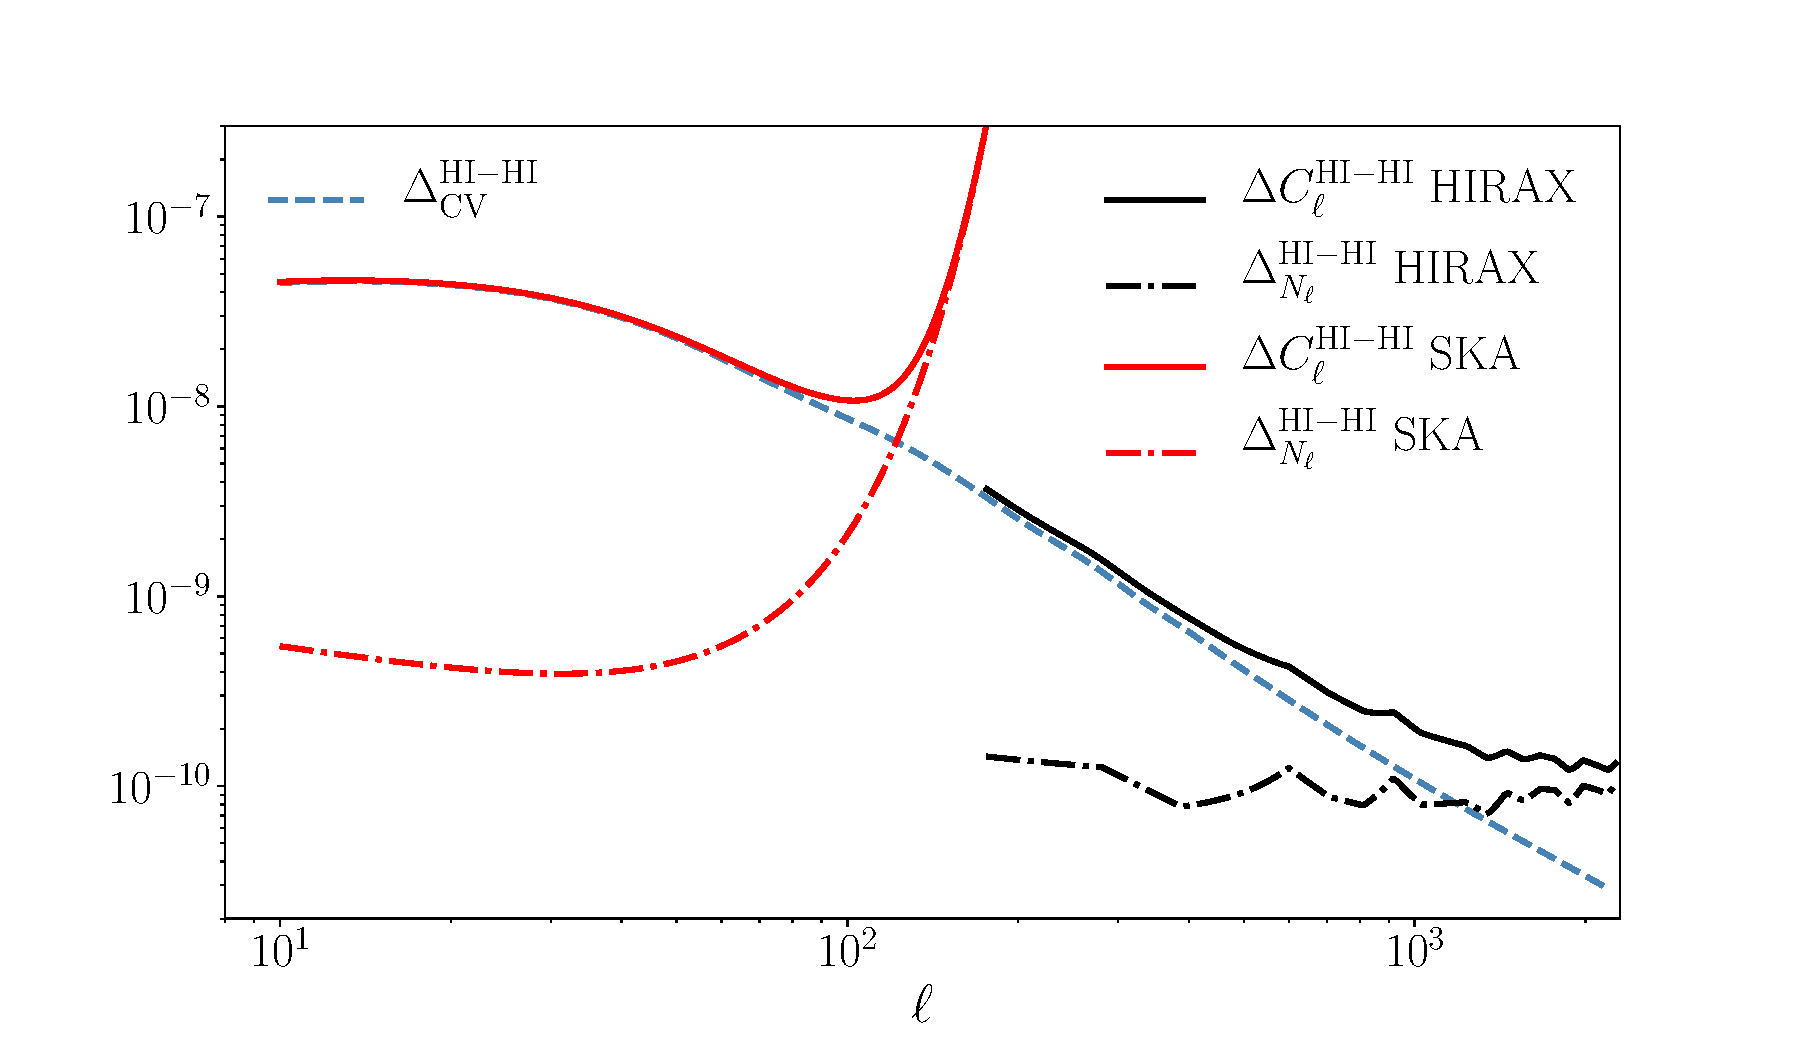
\includegraphics[width=0.95\columnwidth]{HIHI_error_contributions.pdf}
% \centering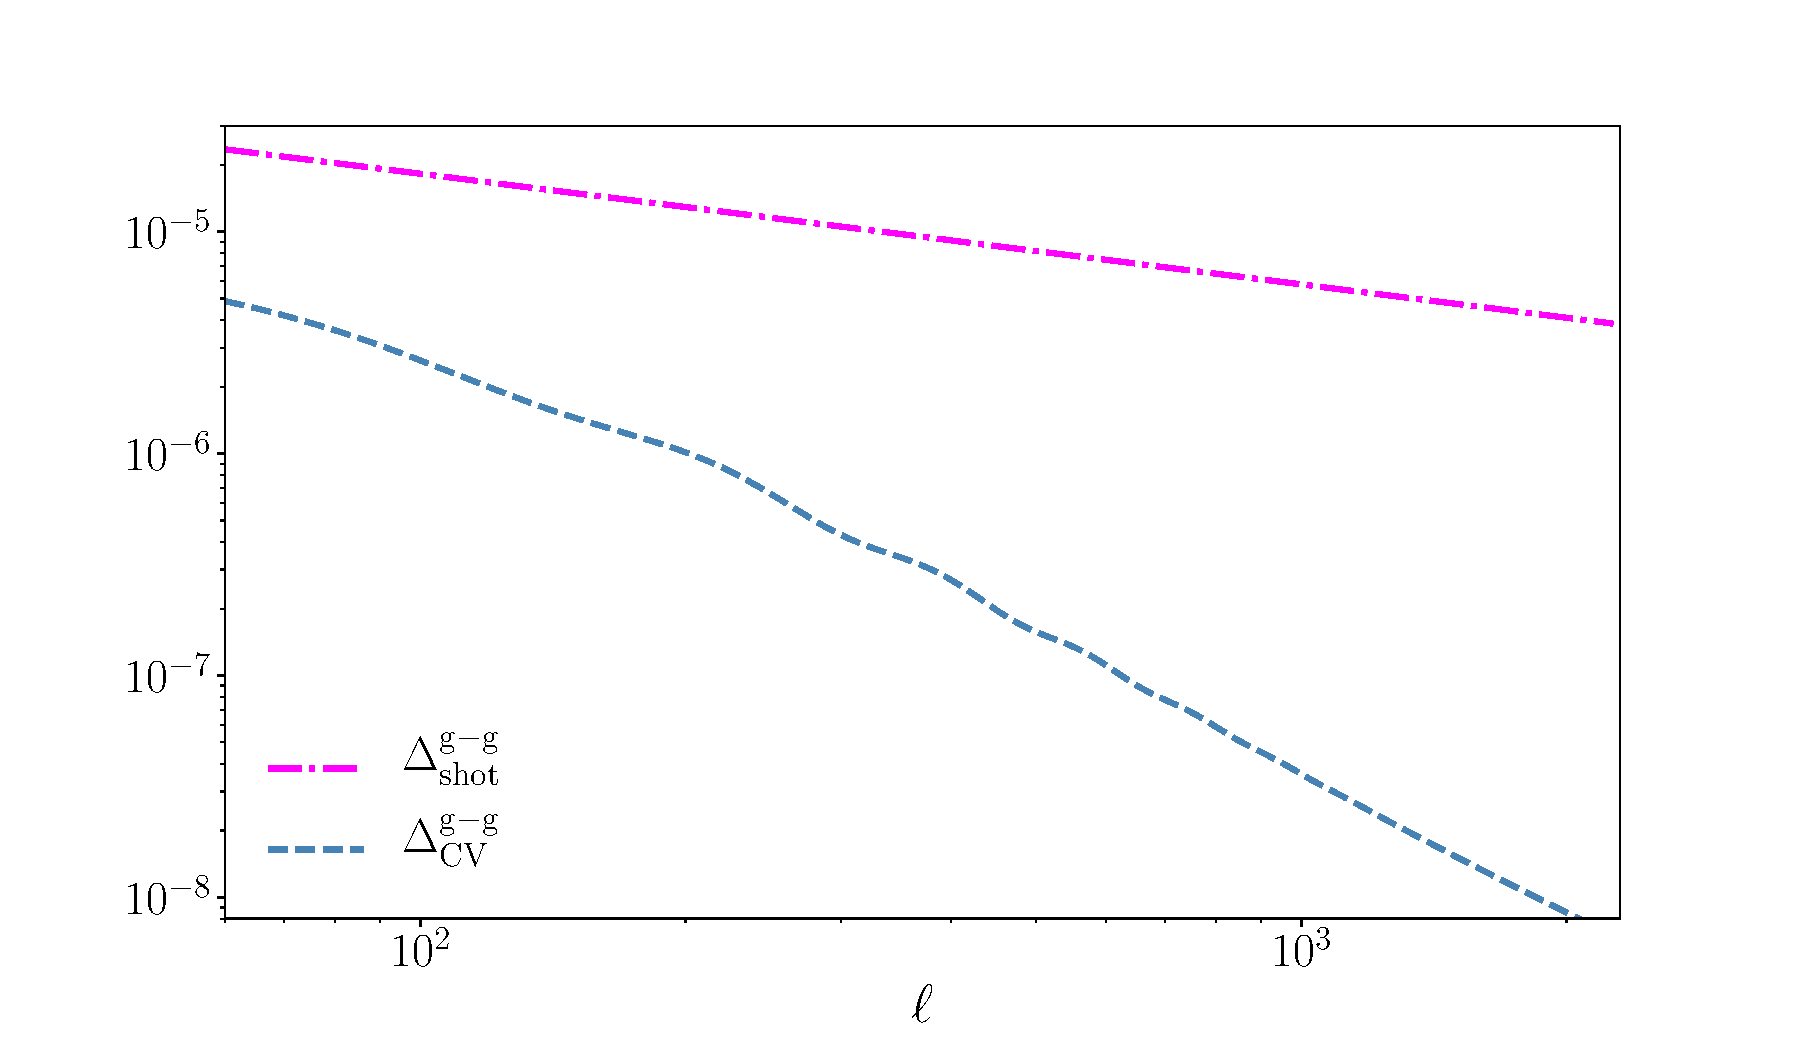
\includegraphics[width=0.95\columnwidth]{GG_error_contributions.pdf}
% % \captionsetup{width=.9\linewidth}

% \centering\caption{{\sl Upper panel:} Contributions to $\Delta C_\ell^{\rm HI-HI}$ as defined in eq. \ref{eq:deltah-h}, for a foreground redshift bin from $z=0.85$ to $1.35$ and a background bin $z\geq1.45$. Note that HIRAX and SKA are sensitive to complimentary scale ranges.
% {\sl Lower panel:} Contributions to $\Delta C_\ell^{\rm g-g}$ as defined in eq. \ref{eq:deltag-g} using the sky fraction for HIRAX, the maximum achievable flux limit for LSST in the redshift bin $z\geq 1.45$. Shot noise dominates at scales $\ell > 10^3$.}
% \label{fig:HIHI_error_contributions}
% \label{fig:gg_error_contributions}
% \end{figure}

% \begin{figure}
% \centering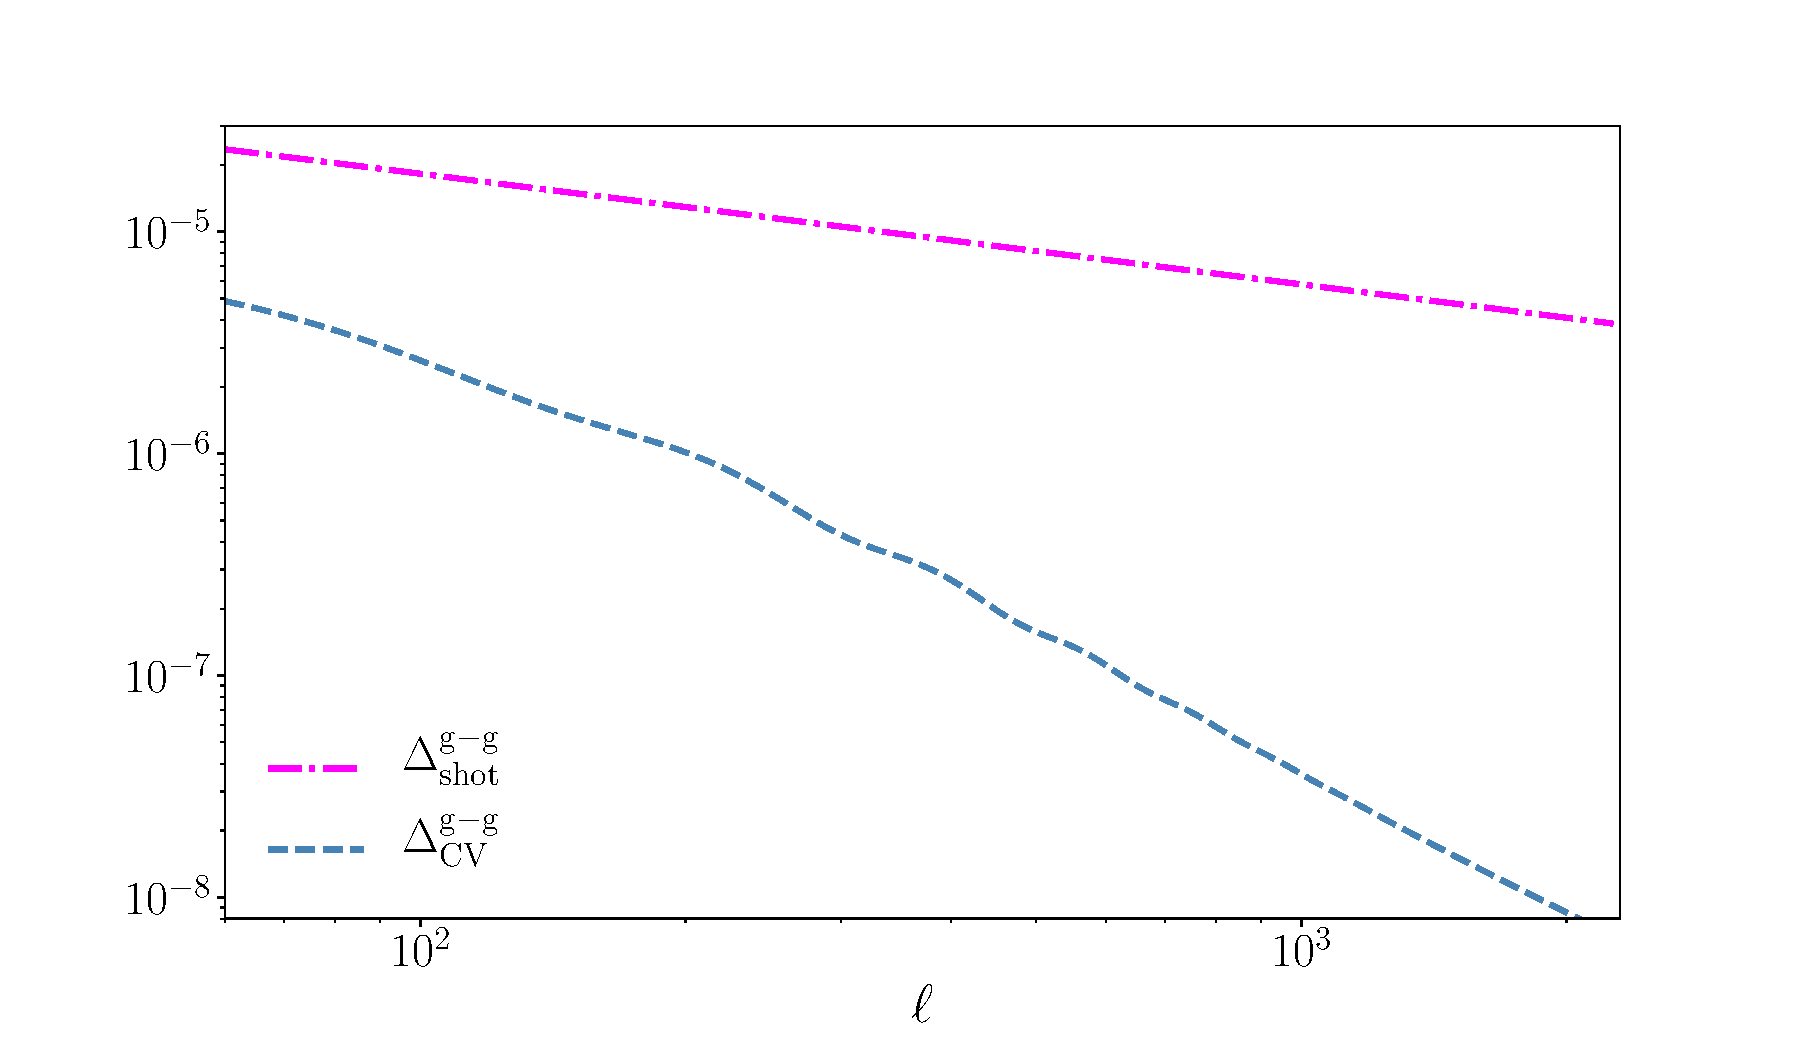
\includegraphics[width=0.85\columnwidth]{GG_error_contributions.pdf}
% \caption{Contributions to $\Delta C_\ell^{\rm g-g}$ as defined in eq. \ref{eq:deltag-g} using the sky fraction for HIRAX, the maximum achievable flux limit for LSST in the redshift bin $z\geq 1.45$. Shot noise dominates at scales $\ell > 10^3$.}
% \label{fig:gg_error_contributions}
% \end{figure}

% Figure \ref{fig:S2N_perfect_galaxies} illustrates the effect of the galaxy shot noise by comparing a perfect galaxy survey to LSST. We plot both cases combined with HIRAX or SKA for one single foreground / background redshift combination each. The forecasts for SKA and HIRAX behave very differently. While the signal to noise for HIRAX benefits immensely from removing the galaxy shot noise, it literally makes no difference to the results for SKA, as these are limited by the single dish noise.

We maximize the signal to noise ratio with respect to the galaxy magnitude threshold $m^*$ for each HI survey and redshift bin. We consider an optimization range of $m^* \in [19,27]$ and plot $\mathrm{S2N}(m^*)$ for a few examples in \ref{fig:S2Nmstar}. The optimal values we found are shown in table \ama{include a table}. Generally, for low-redshift foreground bins, also a low $m^*$ is preferred, which increases the number count slope at the acceptable cost of increasing the negligible shot-noise. For high-redshift foreground bins, however, shot-noise increases and $m^*$ needs to be higher to account for this.

Figure \ref{fig:S2N} shows the optimized signal to noise as a function of redshift for all considered experiment combinations. Maps in each foreground redshift bin are correlated with one single, non-overlapping redshift bin of LSST. Low redshift foreground bins benefit from a wider background sample containing a larger number of galaxies. Therefore, they often perform better than high redshift bins, especially in the case for HIRAX, where the LSST shot noise is clearly the dominant source of error. The sensitivity of HIRAX is best at comparably small scales, where the power spectrum drops $\sim \ell^2$ (see e.g. fig. \ref{fig:HIxmag_Cls}). The shot noise, however, becomes the dominant error on smaller scales. The 512 dish design for HIRAX performs surprisingly well, as even in this case the interferometer noise remains subdominant. We follow \cite{Smith:2002dz} to calculate the nonlinear scale $k_{\rm NL}(z) = k_{\rm NL,0} (1+z)^{2/(2+n_{\rm s})}$, where $n_{\rm s}$ is the spectral index of primordial scalar perturbations, and $k_{\rm NL,0} = 0.14$ Mpc${}^{-1}$ and discard all information from non-linear scales. Figure \ref{fig:S2N_cum} shows the cumulative signal to noise which reaches levels of \ama{finalize} for individual redshift bins. The performance of SKA and HIRAX is similar for individual $\ell$'s, but the better $\ell$ resolution of SKA increases its cumulative signal to noise level well past HIRAX. As both experiments are sensitive to different multipole ranges, most of their constraining power can be combined even at the same redshifts.


An illustration of the different sources of error in the ${\rm HI}-\mu$ power spectrum is shown in figure \ref{fig:x_error_contributions}. To ease comparison we used the same single redshift bin for HIRAX and SKA, from $z=0.85$ to $1.35$. For HIRAX the optimal cutoff is $m^* = 24.4$ and for SKA it is 24.3. While on large scales cosmic variance dominates for all power spectra, both ${\rm HI}-\mu$ and ${\rm HI-HI}$ are dominated by the finite beam width on smaller scales, SKA being limited to much larger scales than HIRAX.
%Let us consider the ``perfect surveys" scenario for the measurement of the HI-$\mu$ signal; that is, we assume $f_{\rm sky}=1$ and we ignore the shot and thermal noise contributions. We assume the HI sample to lie along a redshift range $0<z<1.5$, and the galaxy sample along $0<z<2$. Since we are dealing with an idealised situation, we model the redshift distributions as delta functions at $z_{\rm f}$ and $z_{\rm b}$; we also consider a $\Delta z = 0.1$ binning.
%Hence we get
%\bea \nonumber
%&&C^{{\rm HI} - \mu}_\ell (z_{\rm f}, z_{\rm b}) = \left(\frac{3}{2}\frac{H^2_0}{c^2}\Omega_{{\rm m},0} \right) b_{\rm HI}(5s^{\rm b}_{\rm g}-2) \\
%&\times& \frac{r(z_{\rm b})-r(z_{\rm f})}{r(z_{\rm f})r(z_{\rm b})} (1+z_{\rm f})P(\ell/r(z_{\rm f}),z_{\rm f}) \, .
%\eea
%For the HI bias we use the fit from \citet{Santos:2015bsa}
%\be
%b_{\rm HI}(z) = 0.67+0.18z+0.05z^2 \, ,
%\ee while for modelling $s_{\rm g}$ we use the fit from \citet{Fonseca:2016xvi}
%\be
%s_{\rm g}(z) = 0.132+0.259z-0.281z^2+0.691z^3-0.409z^4+0.152z^5 \, ,
%\ee which was calculated assuming a photometric optical galaxy survey similar to DES.

%\begin{figure}
%\includegraphics[scale=0.6]{CTHI.pdf}
%\caption{The angular spectrum of the correlation of the Planck CMB temperature at $z_c=0.5$ (solid black line) and $z_c=1.2$ (dashed black line) for our fiducial cosmology. The bin width is $\Delta z =0.1$.}
%\label{fig:CTHI}
%\end{figure}





\section{Discussion}
This work demonstrates that, due to their complimentary multipole ranges of sensitivity, instruments like SKA1 MID, HIRAX and LSST combine well for a magnification bias detection. We derived predictions for the signal to noise ratio of the magnification signal from foreground HI maps acting on the clustering of background galaxies, using the optimal galaxy magnitude threshold $m^*$ for LSST. We considered the survey combinations HIRAX with LSST and SKA1 MID with LSST. Due to their different resolutions, the information provided by the interferometer HIRAX is complimentary to the data gathered by SKA in autocorrelation mode. A detection seems likely with forecasted cumulative signal to noise ratios in the range of \ama{finalize}, but a more detailed analysis will be needed to fully assess all relevant sources of errors, e.g. foreground contamination residuals and cleaning effects. Foreground residuals are not expected to be significant in the cross-correlation between HI intensity maps and galaxies, and the loss of long-wavelength radial modes in the HI data is also not expected to have a significant deteriorating effect. The choice of redshift binning could be reconsidered, making the analysis more realistic for a foreground cleaned HI survey, and potentially also improving the signal.


%\section*{Acknowledgments}
%%%%%%%%%%

% \bibliographystyle{mn2e}
\bibliographystyle{mnras}
\bibliography{magnification_IM}


\end{document}
